\documentclass[10pt,journal,compsoc]{IEEEtran}

\usepackage{graphicx}
\usepackage{hyperref}
\usepackage{multirow}
\usepackage{booktabs}
\usepackage{float}
\usepackage{placeins}
\usepackage{bbm}
\usepackage{dsfont}
\usepackage{eufrak}
\usepackage{color}


\bibliographystyle{unsrt}

%
\ifCLASSOPTIONcompsoc
  % IEEE Computer Society needs nocompress option
  % requires cite.sty v4.0 or later (November 2003)
  \usepackage[nocompress]{cite}
\else
  % normal IEEE
  \usepackage{cite}
\fi
% cite.sty was written by Donald Arseneau
% V1.6 and later of IEEEtran pre-defines the format of the cite.sty package
% \cite{} output to follow that of the IEEE. Loading the cite package will
% result in citation numbers being automatically sorted and properly
% "compressed/ranged". e.g., [1], [9], [2], [7], [5], [6] without using
% cite.sty will become [1], [2], [5]--[7], [9] using cite.sty. cite.sty's
% \cite will automatically add leading space, if needed. Use cite.sty's
% noadjust option (cite.sty V3.8 and later) if you want to turn this off
% such as if a citation ever needs to be enclosed in parenthesis.
% cite.sty is already installed on most LaTeX systems. Be sure and use
% version 5.0 (2009-03-20) and later if using hyperref.sty.
% The latest version can be obtained at:
% http://www.ctan.org/pkg/cite
% The documentation is contained in the cite.sty file itself.
%
% Note that some packages require special options to format as the Computer
% Society requires. In particular, Computer Society  papers do not use
% compressed citation ranges as is done in typical IEEE papers
% (e.g., [1]-[4]). Instead, they list every citation separately in order
% (e.g., [1], [2], [3], [4]). To get the latter we need to load the cite
% package with the nocompress option which is supported by cite.sty v4.0
% and later. Note also the use of a CLASSOPTION conditional provided by
% IEEEtran.cls V1.7 and later.





% *** GRAPHICS RELATED PACKAGES ***
%
\ifCLASSINFOpdf
  % \usepackage[pdftex]{graphicx}
  % declare the path(s) where your graphic files are
  % \graphicspath{{../pdf/}{../jpeg/}}
  % and their extensions so you won't have to specify these with
  % every instance of \includegraphics
  % \DeclareGraphicsExtensions{.pdf,.jpeg,.png}
\else
  % or other class option (dvipsone, dvipdf, if not using dvips). graphicx
  % will default to the driver specified in the system graphics.cfg if no
  % driver is specified.
  % \usepackage[dvips]{graphicx}
  % declare the path(s) where your graphic files are
  % \graphicspath{{../eps/}}
  % and their extensions so you won't have to specify these with
  % every instance of \includegraphics
  % \DeclareGraphicsExtensions{.eps}
\fi
% graphicx was written by David Carlisle and Sebastian Rahtz. It is
% required if you want graphics, photos, etc. graphicx.sty is already
% installed on most LaTeX systems. The latest version and documentation
% can be obtained at:
% http://www.ctan.org/pkg/graphicx
% Another good source of documentation is "Using Imported Graphics in
% LaTeX2e" by Keith Reckdahl which can be found at:
% http://www.ctan.org/pkg/epslatex
%
% latex, and pdflatex in dvi mode, support graphics in encapsulated
% postscript (.eps) format. pdflatex in pdf mode supports graphics
% in .pdf, .jpeg, .png and .mps (metapost) formats. Users should ensure
% that all non-photo figures use a vector format (.eps, .pdf, .mps) and
% not a bitmapped formats (.jpeg, .png). The IEEE frowns on bitmapped formats
% which can result in "jaggedy"/blurry rendering of lines and letters as
% well as large increases in file sizes.
%
% You can find documentation about the pdfTeX application at:
% http://www.tug.org/applications/pdftex






% *** MATH PACKAGES ***
%
%\usepackage{amsmath}
% A popular package from the American Mathematical Society that provides
% many useful and powerful commands for dealing with mathematics.
%
% Note that the amsmath package sets \interdisplaylinepenalty to 10000
% thus preventing page breaks from occurring within multiline equations. Use:
%\interdisplaylinepenalty=2500
% after loading amsmath to restore such page breaks as IEEEtran.cls normally
% does. amsmath.sty is already installed on most LaTeX systems. The latest
% version and documentation can be obtained at:
% http://www.ctan.org/pkg/amsmath





% *** SPECIALIZED LIST PACKAGES ***
%
%\usepackage{algorithmic}
% algorithmic.sty was written by Peter Williams and Rogerio Brito.
% This package provides an algorithmic environment fo describing algorithms.
% You can use the algorithmic environment in-text or within a figure
% environment to provide for a floating algorithm. Do NOT use the algorithm
% floating environment provided by algorithm.sty (by the same authors) or
% algorithm2e.sty (by Christophe Fiorio) as the IEEE does not use dedicated
% algorithm float types and packages that provide these will not provide
% correct IEEE style captions. The latest version and documentation of
% algorithmic.sty can be obtained at:
% http://www.ctan.org/pkg/algorithms
% Also of interest may be the (relatively newer and more customizable)
% algorithmicx.sty package by Szasz Janos:
% http://www.ctan.org/pkg/algorithmicx




% *** ALIGNMENT PACKAGES ***
%
%\usepackage{array}
% Frank Mittelbach's and David Carlisle's array.sty patches and improves
% the standard LaTeX2e array and tabular environments to provide better
% appearance and additional user controls. As the default LaTeX2e table
% generation code is lacking to the point of almost being broken with
% respect to the quality of the end results, all users are strongly
% advised to use an enhanced (at the very least that provided by array.sty)
% set of table tools. array.sty is already installed on most systems. The
% latest version and documentation can be obtained at:
% http://www.ctan.org/pkg/array


% IEEEtran contains the IEEEeqnarray family of commands that can be used to
% generate multiline equations as well as matrices, tables, etc., of high
% quality.




% *** SUBFIGURE PACKAGES ***
%\ifCLASSOPTIONcompsoc
%  \usepackage[caption=false,font=footnotesize,labelfont=sf,textfont=sf]{subfig}
%\else
%  \usepackage[caption=false,font=footnotesize]{subfig}
%\fi
% subfig.sty, written by Steven Douglas Cochran, is the modern replacement
% for subfigure.sty, the latter of which is no longer maintained and is
% incompatible with some LaTeX packages including fixltx2e. However,
% subfig.sty requires and automatically loads Axel Sommerfeldt's caption.sty
% which will override IEEEtran.cls' handling of captions and this will result
% in non-IEEE style figure/table captions. To prevent this problem, be sure
% and invoke subfig.sty's "caption=false" package option (available since
% subfig.sty version 1.3, 2005/06/28) as this is will preserve IEEEtran.cls
% handling of captions.
% Note that the Computer Society format requires a sans serif font rather
% than the serif font used in traditional IEEE formatting and thus the need
% to invoke different subfig.sty package options depending on whether
% compsoc mode has been enabled.
%
% The latest version and documentation of subfig.sty can be obtained at:
% http://www.ctan.org/pkg/subfig




% *** FLOAT PACKAGES ***
%
%\usepackage{fixltx2e}
% fixltx2e, the successor to the earlier fix2col.sty, was written by
% Frank Mittelbach and David Carlisle. This package corrects a few problems
% in the LaTeX2e kernel, the most notable of which is that in current
% LaTeX2e releases, the ordering of single and double column floats is not
% guaranteed to be preserved. Thus, an unpatched LaTeX2e can allow a
% single column figure to be placed prior to an earlier double column
% figure.
% Be aware that LaTeX2e kernels dated 2015 and later have fixltx2e.sty's
% corrections already built into the system in which case a warning will
% be issued if an attempt is made to load fixltx2e.sty as it is no longer
% needed.
% The latest version and documentation can be found at:
% http://www.ctan.org/pkg/fixltx2e


%\usepackage{stfloats}
% stfloats.sty was written by Sigitas Tolusis. This package gives LaTeX2e
% the ability to do double column floats at the bottom of the page as well
% as the top. (e.g., "\begin{figure*}[!b]" is not normally possible in
% LaTeX2e). It also provides a command:
%\fnbelowfloat
% to enable the placement of footnotes below bottom floats (the standard
% LaTeX2e kernel puts them above bottom floats). This is an invasive package
% which rewrites many portions of the LaTeX2e float routines. It may not work
% with other packages that modify the LaTeX2e float routines. The latest
% version and documentation can be obtained at:
% http://www.ctan.org/pkg/stfloats
% Do not use the stfloats baselinefloat ability as the IEEE does not allow
% \baselineskip to stretch. Authors submitting work to the IEEE should note
% that the IEEE rarely uses double column equations and that authors should try
% to avoid such use. Do not be tempted to use the cuted.sty or midfloat.sty
% packages (also by Sigitas Tolusis) as the IEEE does not format its papers in
% such ways.
% Do not attempt to use stfloats with fixltx2e as they are incompatible.
% Instead, use Morten Hogholm'a dblfloatfix which combines the features
% of both fixltx2e and stfloats:
%
% \usepackage{dblfloatfix}
% The latest version can be found at:
% http://www.ctan.org/pkg/dblfloatfix




%\ifCLASSOPTIONcaptionsoff
%  \usepackage[nomarkers]{endfloat}
% \let\MYoriglatexcaption\caption
% \renewcommand{\caption}[2][\relax]{\MYoriglatexcaption[#2]{#2}}
%\fi
% endfloat.sty was written by James Darrell McCauley, Jeff Goldberg and
% Axel Sommerfeldt. This package may be useful when used in conjunction with
% IEEEtran.cls'  captionsoff option. Some IEEE journals/societies require that
% submissions have lists of figures/tables at the end of the paper and that
% figures/tables without any captions are placed on a page by themselves at
% the end of the document. If needed, the draftcls IEEEtran class option or
% \CLASSINPUTbaselinestretch interface can be used to increase the line
% spacing as well. Be sure and use the nomarkers option of endfloat to
% prevent endfloat from "marking" where the figures would have been placed
% in the text. The two hack lines of code above are a slight modification of
% that suggested by in the endfloat docs (section 8.4.1) to ensure that
% the full captions always appear in the list of figures/tables - even if
% the user used the short optional argument of \caption[]{}.
% IEEE papers do not typically make use of \caption[]'s optional argument,
% so this should not be an issue. A similar trick can be used to disable
% captions of packages such as subfig.sty that lack options to turn off
% the subcaptions:
% For subfig.sty:
% \let\MYorigsubfloat\subfloat
% \renewcommand{\subfloat}[2][\relax]{\MYorigsubfloat[]{#2}}
% However, the above trick will not work if both optional arguments of
% the \subfloat command are used. Furthermore, there needs to be a
% description of each subfigure *somewhere* and endfloat does not add
% subfigure captions to its list of figures. Thus, the best approach is to
% avoid the use of subfigure captions (many IEEE journals avoid them anyway)
% and instead reference/explain all the subfigures within the main caption.
% The latest version of endfloat.sty and its documentation can obtained at:
% http://www.ctan.org/pkg/endfloat
%
% The IEEEtran \ifCLASSOPTIONcaptionsoff conditional can also be used
% later in the document, say, to conditionally put the References on a
% page by themselves.




% *** PDF, URL AND HYPERLINK PACKAGES ***
%
%\usepackage{url}
% url.sty was written by Donald Arseneau. It provides better support for
% handling and breaking URLs. url.sty is already installed on most LaTeX
% systems. The latest version and documentation can be obtained at:
% http://www.ctan.org/pkg/url
% Basically, \url{my_url_here}.





% *** Do not adjust lengths that control margins, column widths, etc. ***
% *** Do not use packages that alter fonts (such as pslatex).         ***
% There should be no need to do such things with IEEEtran.cls V1.6 and later.
% (Unless specifically asked to do so by the journal or conference you plan
% to submit to, of course. )


% correct bad hyphenation here
\hyphenation{op-tical net-works semi-conduc-tor}

\usepackage{bm}
\usepackage{amsmath}
\usepackage{amsfonts}


\makeatletter
\newcommand{\printfnsymbol}[1]{%
  \textsuperscript{\@fnsymbol{#1}}%
}
\makeatother

\begin{document}
% \textsuperscript{\dag}
\title{Dynamic Neural Networks: A Survey}
\author{Yizeng~Han\IEEEauthorrefmark{1},
        Gao~Huang\IEEEauthorrefmark{1},~\IEEEmembership{Member,~IEEE,}
        Shiji~Song,~\IEEEmembership{Senior~Member,~IEEE,}
        Le~Yang,
        Honghui~Wang,
        and~Yulin~Wang
         % <-this % stops a space
\IEEEcompsocitemizethanks{\IEEEcompsocthanksitem Yizeng Han, Gao Huang, Shiji Song, Le Yang, Honghui Wang and Yulin Wang are with the Department of Automation, Tsinghua University, Beijing 100084, China. Gao Huang is also with Beijing Academy of Artificial Intelligence, Beijing, 100084. E-mail: \{hanyz18, yangle15, wanghh20, wang-yl19\}@mails.tsinghua.edu.cn; \{gaohuang, shijis\}@tsinghua.edu.cn. Corresponding author: Gao Huang.
% Le Yang is with the School of Information and Communications Engineering, Xi'an Jiaotong University, Xi'an 710049, China. Email: yangle15@xjtu.edu.cn.
}% <-this % stops an unwanted space
%\thanks{Manuscript received April 19, 2005; revised August 26, 2015.}
}
%E-mail: see http://www.michaelshell.org/contact.html

% \markboth{IEEE TRANSACTIONS ON PATTERN ANALYSIS AND MACHINE INTELLIGENCE,~Vol.~XX, No.~XX, XXX~201x}%
% {Li \MakeLowercase{\textit{et al.}}: Discriminative Transfer Feature Learning and Label Consistency for Visual Domain Adaptation}

\IEEEtitleabstractindextext{%
\vskip -0.15in
\begin{abstract}
    
    % Despite the great success achieved by deep neural networks, inference efficiency is still an essential bottleneck limiting their applicability on resource-constrained platforms. 

    % Dynamic neural network is an emerging research topic in deep learning. Compared to static models which have fixed computational graphs and parameters at the inference stage, dynamic networks can adapt their structures or parameters to different inputs, 
    % Efficient inference of deep neural networks has been studied from a variety of perspectives.
    % Traditional methods either conduct post-processing on given models to reduce redundant computations, or directly design lightweight network architectures with low computational cost. However, both solutions keep the computational graphs and model parameters \emph{fixed} after training, treating different input samples with uniform computations. Such \emph{static} inference paradigm induces intrinsic redundancy. Recently, a significant amount of research efforts are made to design various types of \emph{dynamic} networks, 
    % leading to notable advantages in terms of accuracy, computational efficiency, adaptiveness, etc.
    %  due to their \emph{data-dependent inference paradigm}. 
    % In this survey, we comprehensively review this rapidly developing area by dividing dynamic networks into three main categories: 1) \emph{instance-wise} dynamic models that process each instance with data-dependent architectures or parameters; 2) \emph{spatial-wise} dynamic networks that conduct adaptive computation with respect to different spatial locations of image data and 3) \emph{temporal-wise} dynamic models that perform adaptive inference along the temporal dimension for sequential data such as videos and texts. The important research problems of dynamic networks, e.g., architecture design, decision making scheme, optimization technique and applications, are reviewed systematically. Finally, we discuss the open problems in this field together with interesting future research directions.

    Dynamic neural network is an emerging research topic in deep learning. Compared to static models which have fixed computational graphs and parameters at the inference stage, dynamic networks can adapt their structures or parameters to different inputs, leading to notable advantages in terms of accuracy, computational efficiency, adaptiveness, etc. In this survey, we comprehensively review this rapidly developing area by dividing dynamic networks into three main categories: 1) {\emph{sample-wise}} dynamic models that process each sample with data-dependent architectures or parameters; 2) \emph{spatial-wise} dynamic networks that conduct adaptive computation with respect to different spatial locations of image data; and 3) \emph{temporal-wise} dynamic models that perform adaptive inference along the temporal dimension for sequential data such as videos and texts. The important research problems of dynamic networks, e.g., architecture design, decision making scheme, optimization technique and applications, are reviewed systematically. Finally, we discuss the open problems in this field together with interesting future research directions.
\end{abstract}
\vskip -0.1in
% Note that keywords are not normally used for peerreview papers.
\begin{IEEEkeywords}
Dynamic networks, Adaptive inference, Efficient inference, Convolutional neural networks.
\end{IEEEkeywords}}
% make the title area
\maketitle
\begingroup\renewcommand\thefootnote{\IEEEauthorrefmark{1}}
\footnotetext{\emph{Equal contribution.}}
\endgroup

% \begingroup\renewcommand\thefootnote{\dag}
% \footnotetext{\emph{Equal contribution.}}
% \endgroup
% \begingroup\renewcommand\thefootnote{\ddag}
% \footnotetext{\emph{Corresponding author.}}
% \endgroup
\IEEEdisplaynontitleabstractindextext
\IEEEpeerreviewmaketitle

\vspace{-2ex}
\IEEEraisesectionheading{\section{Introduction}\label{sec:introduction}}
% \vskip -0.1in
\IEEEPARstart{D}{eep} neural networks (DNNs) are playing an important role in various areas including computer vision (CV) \cite{alexnet,Simonyan15,szegedy2015going,he2016deep,huang2017densely} and natural language processing (NLP) \cite{vaswani2017attention,devlin_bert_2019,brown2020language}. 
% \IEEEPARstart{D}{eep} learning is playing an important role in cv nlp speech, etc. 
Recent years have witnessed many successful deep models such as AlexNet \cite{alexnet}, VGG \cite{Simonyan15}, GoogleNet \cite{szegedy2015going}, ResNet \cite{he2016deep}, DenseNet \cite{huang2017densely} and Transformer \cite{vaswani2017attention}. These {architectural innovations} have enabled the training of deeper, more accurate and more efficient models. The recent research on neural architecture search (NAS) \cite{zoph2016neural, liu_darts_2018} further speeds up the process of designing more powerful structures. However, most of the prevalent deep learning models perform inference in a static manner, i.e., both the computational graph and the network parameters are fixed once trained, which may limit their representation power, efficiency and interpretability \cite{graves2016adaptive,huang2017multi,yang2019condconv,sabour2017dynamic}. 

Dynamic networks, as opposed to static ones, can adapt their structures or parameters to the input during inference, and therefore enjoy favorable properties that are absent in static models. In general, dynamic computation in the context of deep learning has the following advantages: 


% \IEEEPARstart{D}{eep} neural networks (DNNs) have shown their dominance across various areas including computer vision (CV) \cite{Simonyan15,szegedy2015going,he2016deep,huang2017densely} and natural language processing (NLP) \cite{vaswani2017attention,devlin_bert_2019,radford2019language}, e.t.c. 
% To achieve state-of-the-art performance, 
% researchers have managed to enlarge the capacity and representation power of deep models by endowing them with unprecedented network depth \cite{Simonyan15,he2016deep,huang2017densely} or width \cite{zagoruyko2016wide}. Unfortunately, under a variety of practical scenarios, 
% the high computational demand of these large models has limited 
% % Even though advances in hardware development have enabled the training of these DNNs, 
% % they still tend to be resource-hungry with high computational demands during inference, 
% their deployment and application on resource-constrained platforms such as mobiles, IoT and wearable devices, e.t.c. Therefore, improving the inference efficiency of DNNs has attracted great research interests in the deep learning community. 
% % been a research challenge in the deep learning community. 

% There have been a variety of studies that effectively reduce the computational cost of DNNs, e.g. network pruning \cite{huang2018condensenet,liu2017learning}, weight quantization \cite{hubara2016binarized}, knowledge distillation \cite{hinton2014distilling} and low-rank approximation \cite{low_rank}, e.t.c. However, most of these methods focus on post-processing deep networks with given structures.  
% % and a more fundamental solution is building efficient models by design from two perspectives: \emph{network architectures} and \emph{inference paradigms}. 
% Although extensive efforts have been made to design lightweight models such as MobileNet \cite{howard2017mobilenets} and ShuffleNet \cite{zhang2018shufflenet}, the networks still follow a static inference paradigm, i.e. after being trained, both the model architectures and parameters are fixed when processing different input instances. In fact, it has been observed \cite{huang2017multi,yang_resolution_2020} that even shallow networks are able to correctly recognize most canonical (`easy') samples.
% % modern deep models with larger and larger capacity are mostly built to correctly recognize those non-canonical samples in large-scale datasets (e.g. ImageNet \cite{krizhevsky2012imagenet} for image classification). 
% Therefore, the traditional static inference paradigm can induce intrinsic computational redundancy as treating both canonical and non-canonical (`hard') samples with uniform computations. 

% From the perspectives of both network architecture and inference paradigms, \emph{dynamic deep neural networks} have shown promising results on efficient inference. By adapting their computational graphs to different input \cite{lin2017runtime,huang2017multi,veit2018convolutional}, dynamic networks can allocate the computations dependent on the input complexity. Moreover, despite the billions of neurons in a human brain, its power consumption can be quite low due to the \emph{conditional} activation of the numerous units and their linkages. Compared with static models, dynamic networks can adapt their inference paradigms to the varying environments by selectively activating different modules (e.g. layers \cite{huang2017multi}, channels \cite{lin2017runtime} or even sub-networks \cite{shazeer2017outrageously}) as needed, which is more similar to human intelligent systems. 

% To summarize, dynamic networks are gaining increasing attention due to their remarkable advantages in the following aspects:
\begin{figure*}
  \centering
  \vspace{-2ex}
    \includegraphics[width=0.875\linewidth]{1_overall.pdf}
    \vskip -0.175in
    \centering\caption{Overview of the survey. {We first review the dynamic networks that perform adaptive computation at three different granularities (i.e. sample-wise, spatial-wise and temporal-wise). Then we summarize the decision making strategy, training technique and applications of dynamic models. Existing open problems in this field together with some future research directions are finally discussed. Best viewed in color.}}
    \label{framework}
    \vspace{-3ex}
\end{figure*}

\textbf{1) Efficiency.} One of the most notable advantages of dynamic networks is that they are able to allocate computations on demand at test time, by selectively activating model components (e.g. layers \cite{huang2017multi}, channels \cite{lin2017runtime} or sub-networks \cite{shazeer2017outrageously}) \emph{conditioned} on the input. Consequently, less computation is spent on canonical samples that are relatively easy to recognize, or on less informative spatial/temporal locations of an input. {In addition to \emph{computational efficiency}, dynamic models have also shown promising results for improving \emph{data efficiency} in the scenario of few-shot learning \cite{bertinetto2016learning,wang2019tafe}.}

% \begin{enumerate}
%     \item The adaptive inference scheme is compatible with the other approaches, e.g. dynamic networks can be directly designed based on the lightweight models, and can also benefit from the model pruning and knowledge distillation techniques;
%     \item By conditioning the computation of a deep model on its inputs, adaptive inference can save a considerable amount of computational cost on some `easy' instances or less important regions, drastically reducing the average inference time;
%     \item Dynamic networks usually have a set of tunable hyper-parameters that control the trade-off between accuracy and efficiency, which can be considered as a valuable property when the computational budget might changes over time or across different platforms, and enable dynamic networks to trade accuracy for speed or vise verse on-the-fly to meet the varying need. This is essentially different from static models with fixed computational cost.
% \end{enumerate}

\textbf{2) Representation power.} Due to the data-dependent network architecture/parameters, dynamic networks have significantly enlarged parameter space and improved representation power. For example, with a minor increase of computation, model capacity can be boosted by applying feature-conditioned attention weights on an ensemble of convolutional kernels \cite{yang2019condconv,chen_dynamic_2020_attentionOver}. It is worth noting that the popular soft attention mechanism could also be unified in the framework of dynamic networks, as different channels \cite{hu2018squeeze}, spatial areas \cite{woo_cbam_2018} or temporal locations \cite{yang_neural_2017} of features are dynamically re-weighted at test time. 
% We can observe that these parameter adaptation methods consistently boost the network performance on a large range of tasks. 
%Compared to static models that adapt their parameters to specific \emph{datasets}, dynamic networks can provide a more suitable approach to encode feature representations by adapting their parameters to each \emph{instance}, and effectively improve the network performance on a large range of tasks.
% which effectively improves the generalization of deep models in real applications.

% \textbf{(3) More suitable for modeling the real-world data diversity.} Indeed, the inference procedure itself is inherently dynamic, which means that various samples do need to be treated in different ways. However, in the conventional machine learning framework, we only adapt the models to each \emph{dataset}, rather than to each \emph{instance}. In other words, we train a network on a specific dataset due to the variance of data distributions among multiple datasets. In fact, the data distribution in a single dataset can be still varying, and real-world samples are even more diverse than those in public datasets. Therefore, dynamic networks provide a suitable approach to model such data diversity: rather than utilizing a static model, it adaptively encodes the feature representations dependent on every instance, which improves the generalization of deep models in real applications.

% \textbf{3) Generality.} Dynamic networks are making fundamental changes to the learning paradigm of deep models by innovations from the perspectives of both network architecture and inference scheme. As a result, dynamic networks are not task-specific, and are general enough to take advantages in a wide range of applications, including vision tasks such as image classification \cite{huang2017multi, yang_resolution_2020}, object detection \cite{figurnov2017spatially} and semantic segmentation \cite{li_not_2017}, e.t.c Moreover, methods developed in CV tasks can transfer well on language models in NLP tasks \cite{dehghani_universal_2019, elbayad_depth-adaptive_2020}, and vice versa.

\textbf{3) Adaptiveness.} Dynamic models are able to achieve a desired trade-off between accuracy and efficiency for dealing with varying computational budgets on the fly. Therefore, they are more adaptable to different hardware platforms and changing environments, compared to static models with a fixed computational cost.

\textbf{4) Compatibility.} Dynamic networks are compatible with most advanced techniques in deep learning, including architecture design \cite{he2016deep,huang2017densely}, optimization algorithms \cite{kingma2014adam,DBLP:journals/corr/IoffeS15} and data preprocessing \cite{wang2019implicit,DBLP:journals/corr/abs-1805-09501}, which ensures that they can benefit from the most recent advances in the field to achieve state-of-the-art performance. For example, dynamic networks can inherit architectural innovations in lightweight models \cite{howard2017mobilenets}, or be designed via NAS approaches \cite{zoph2016neural, liu_darts_2018}. Their efficiency could also be further improved by acceleration methods developed for static models, such as network pruning \cite{huang2018condensenet}, weight quantization \cite{hubara2016binarized}, knowledge distillation \cite{hinton2014distilling} and low-rank approximation \cite{low_rank}.

\textbf{5) Generality.} As a substitute for static deep learning techniques, many dynamic models are general approaches that can be applied seamlessly to a wide range of applications, such as image classification \cite{huang2017multi, yang_resolution_2020}, object detection \cite{figurnov2017spatially} and semantic segmentation \cite{li_not_2017}. Moreover, the techniques developed in CV tasks are proven to transfer well to language models in NLP tasks \cite{dehghani_universal_2019, elbayad_depth-adaptive_2020}, and vice versa.


\textbf{6) Interpretability.} We finally note that the research on dynamic networks {may bridge} the gap between the underlying mechanism of deep models and brains, as it is believed that the brains process information in a dynamic way~\cite{hubel1962receptive,murata2000selectivity}. It is possible to analyze which components of a dynamic model are activated \cite{yang_resolution_2020} when processing an input sample, and to observe which parts of the input are accountable for certain predictions \cite{wang2020glance}. These properties may shed light on interpreting the decision process of DNNs.


% We finally note that the brains process information in a dynamic way~\cite{hubel1962receptive,murata2000selectivity}. 
% The research on dynamic networks may potentially bridge the gap between the underlying mechanism of deep models and brains, providing better interpretability for DNNs. In dynamic models, it is feasible to analyze which components of a network are activated \cite{yang_resolution_2020} when processing an input instance. Such adaptive computation corresponds to the conditional activation of neurons in brains~\cite{hubel1962receptive,murata2000selectivity}. In addition, for spatial-wise adaptive models, one can easily observe which parts of the input are essential for the network to generate its predictions \cite{wang2020glance}.

% despite the billions of neurons in a human brain, its power consumption can be quite low due to the \emph{conditional} activation of the numerous units and their linkages. Compared with static models, dynamic networks can adapt their inference paradigms to the varying environments by selectively activating different modules () as needed, which is more similar to human intelligent systems. 

\begin{table}
  \vspace{-1ex}
  \caption{Notations used in this paper.}
  \label{tab:notations}
  \vspace{-4ex}
  \begin{center}
    \begin{tabular}{c|c}
      \hline
      \textbf{Notations} & \textbf{Descriptions} \\
      \hline
      $\mathbb{R}^m$ & $m$-dimensional real number domain \\
      \hline
      % $\mathbb{Z}^m$ & $m$-dimensional integer number domain \\
      % \hline
      $a, \mathbf{a}$ & Scalar, vector/matrix/tensor \\
      \hline
      $\mathbf{x,y}$ & Input, output feature \\
      \hline
      $\mathbf{x}^{\ell}$ & Feature at layer $\ell$ \\
      \hline
      $\mathbf{h}_t$ & Hidden state at time step $t$ \\
      \hline
      % $\mathbf{\tilde{x}}$ & Attention-gated features \\
      % \hline
      $\mathbf{x(p)}$ & Feature at spatial location $\mathbf{p}$ on $\mathbf{x}$ \\
      \hline
      $\bm{\Theta}$ & Learnable parameter \\
      \hline
      $\bm{\hat{\Theta}}|\mathbf{x}$ & Dynamic parameter conditioned on $\mathbf{x}$ \\
      \hline
      $\mathbf{x}\star\mathbf{W}$ & Convolution of feature $\mathbf{x}$ and weight $\mathbf{W}$ \\
      \hline
      $\otimes$ & Channel-wise or element-wise multiplication \\
      \hline
      $\mathcal{F}(\cdot,\bm{\Theta})$ & Functional Operation parameterized by $\bm{\Theta}$ \\
      \hline
      $\mathcal{F}\circ\mathcal{G}$ & Composition of function $\mathcal{F}$ and $\mathcal{G}$ \\
      \hline
      % $\mathrm{FC}(\cdot)$ & Fully connected layer \\
      % \hline
      % $\mathrm{GAP}(\cdot)$ & Global Average Pooling \\
      % \hline
      % $\sigma(\cdot)$ & The sigmoid function \\
      % \hline
      % $\mathrm{ReLU}(\cdot)$ & The ReLU activation function \\
      % \hline
      % $\mathrm{Tanh}(\cdot)$ & The hyperbolic tangent function \\
      % \hline
    \end{tabular}
  \end{center}
  \vskip -0.35in
\end{table}

In fact, adaptive inference, the key idea underlying dynamic networks, has been studied before the popularity of modern DNNs. The most classical approach is building a model ensemble through a cascaded \cite{viola_robust_2004} or parallel \cite{jacobs1991adaptive} structure, and selectively activating the models conditioned on the input. Spiking neural networks (SNNs) \cite{maass1997networks,izhikevich2003simple} also perform data-dependent inference by propagating pulse signals. However, the training strategy for SNNs is quite different from that of popular convolutional neural networks (CNNs), and they are less used in vision tasks. Therefore, we leave out the work related to SNNs in this survey. 
% For example, in classical machine learning approaches like decision trees \cite{quinlan1986induction}, the inference procedure is naturally dynamic, as every sample is routed along a data-dependent path inside the tree. It has also been studied to achieve 

\begin{figure}
  \centering
    \vspace{-1ex}
    \includegraphics[width=\linewidth]{2_dynamic_cascade.pdf}
    \vskip -0.15in
    \caption{Two early-exiting schemes. The dashed lines and shaded modules are not executed, conditioned on the decisions made by the routers.}
    \label{cascading_models}
    \vskip -0.2in
\end{figure}
% \cite{jacobs1991adaptive} achieves an adaptive mixture of multiple feedforward networks with a gating module; \cite{schmidhuber1992learning} builds a system with one feedforward network predicting the weight changes for the other one; spiking neural network (SNN) \cite{maass1997networks,izhikevich2003simple} propagates pulse signals to conditionally activate its neurons based on the input; \cite{rowley1998neural} uses a cascaded structure to quickly eliminate negative samples for face detection; \cite{gao2011active} and \cite{karayev_timely_2012} achieve adaptive inference for classification and object detection respectively based on traditional machine learning models.

\begin{figure*}
  \centering
  \vspace{-2ex}
    \includegraphics[width=\linewidth]{3_multi_scale_SuperNet.pdf}
    \vskip -0.175in
    \caption{{Multi-scale architectures with dynamic inference graphs. The first three models (a, b, c) perform adaptive early exiting with specific architecture designs and exiting policies. Dynamic routing is achieved inside a SuperNet (d) to activate data-dependent inference paths.}}
    \label{multi_scale}
    \vspace{-3ex}
\end{figure*}
In the context of deep learning, dynamic inference with modern deep architectures, has raised many new research questions and has attracted great research interests in the past three years.
% Inspired by the aforementioned early studies, numerous forms of dynamic networks \cite{lin2017runtime,huang2017multi,veit2018convolutional,hu2018squeeze,dai2017deformable} have been designed by exploiting advanced deep learning techniques. 
Despite the extensive work on designing various types of dynamic networks, a systematic and comprehensive review on this topic is still lacking. This motivates us to write this survey, to review the recent advances in this rapidly developing area, with the purposes of 1) providing an overview as well as new perspectives for researchers who are interested in this topic; 2) pointing out the close relations of different subareas and reducing the risk of reinventing the wheel; and 3) summarizing the key challenges and possible future research directions.


{This survey is organized as follows (see \figurename~\ref{framework} for an overview). In Sec. \ref{sec_sample_wise}, we introduce the most common \emph{sample-wise} dynamic networks which adapt their architectures or parameters conditioned on each input sample. Dynamic models working on a finer granularity, i.e., \emph{spatially} adaptive and \emph{temporally} adaptive models, are reviewed in Sec. \ref{sec_spatially_adaptive} and Sec.\ref{sec_temporal_adaptive}, respectively\footnote{{These two categories can also be viewed as sample-wise dynamic networks as they perform adaptive computation within each sample at a finer granularity, and we adopt such a split for narrative convenience.}}. Then we investigate the decision making strategies and the training techniques of dynamic networks in Sec. \ref{inference_and_train}. The applications of dynamic models are further summarized in Sec. \ref{sec_tasks}. Finally, we conclude this survey with a discussion on a number of open problems and future research directions in Sec. \ref{sec:discussion}. For better readability, we list the notations that will be used in this survey in Table \ref{tab:notations}.}

\vspace{-2ex}
% \input{2_why.tex}
% \vspace{-2ex}
% \input{2_how.tex}
% \vspace{-2ex}
\section{{Sample-wise Dynamic Networks}}
\label{sec_sample_wise}
Aiming at processing different inputs in data-dependent manners, sample-wise dynamic networks are typically designed from two perspectives: 1) adjusting model architectures to allocate appropriate computation based on each sample, and therefore reducing redundant computation for increased efficiency (Sec. \ref{dynamic_arch}); 
  % adjusting model \emph{architectures} conditioned on each sample, to improve the inference efficiency with decent accuracy sacrifice (Sec. \ref{dynamic_arch})}; 
2) adapting network \emph{parameters} to every input sample with fixed computational graphs, with the goal of boosting the representation power with minimal increase of computational cost (Sec. \ref{adaptive_params}).
% For example, an adaptive ensemble of classifiers based on their output values is implemented in \cite{gao2011active}, and \cite{karayev_timely_2012} sequentially employs one selected detector to conduct timely object detection. These approaches 
% mostly make breakthroughs towards dynamic inference schemes based on traditional model architectures, and 


\vspace{-2ex}
\subsection{Dynamic Architectures}
\label{dynamic_arch}
% \vspace{-0.5ex}
Considering different inputs may have diverse computational demands, it is natural to perform inference with dynamic architectures conditioned on each sample. Specifically, one can adjust the network depth (Sec. \ref{dynamic_depth}), width (Sec. \ref{dynamic_width}), or perform dynamic routing within a super network (SuperNet) that includes multiple possible paths (Sec. \ref{SuperNets}). Networks with dynamic architectures not only save redundant computation for canonical ("easy") samples, but also preserve their representation power when recognizing non-canonical ("hard") samples. Such a property leads to remarkable advantages in efficiency compared to the acceleration techniques for static models \cite{huang2018condensenet,liu2017learning, hubara2016binarized}, which handle "easy" and "hard" inputs with identical computation, and fail to reduce intrinsic computational redundancy.

\vspace{-1.5ex}
\subsubsection{Dynamic Depth} \label{dynamic_depth}
As modern DNNs are getting increasingly deep for recognizing more "hard" samples, a straightforward solution to reducing redundant computation is performing inference with dynamic depth, which can be realized by 1) \emph{early exiting}, i.e. allowing "easy" samples to be output at shallow exits without executing deeper layers \cite{teerapittayanon2016branchynet,bolukbasi2017adaptive,huang2017multi}; or 2) \emph{layer skipping}, i.e. selectively skipping intermediate layers conditioned on each sample \cite{graves2016adaptive,wang2018skipnet,veit2018convolutional}.
% Due to the sequential execution procedure of deep networks, models with dynamic depths usually enjoy favorable runtime efficiency in practice.
%  on various tasks especially classification.

\begin{figure*}
  \vspace{-2ex}
  \centering
    \includegraphics[width=\linewidth]{4_skip_layers.pdf}
    \vskip -0.175in
    \caption{Dynamic layer skipping. Feature $\mathbf{x}_4$ in (a) are not calculated conditioned on the halting score, and the gating module in (b) decides whether to execute the block based on the intermediate feature. The policy network in (c) generates the skipping decisions for all layers in the main network.}
    \label{skipping_layers}
    \vspace{-3ex}
\end{figure*}
\noindent\textbf{1) Early exiting.} The complexity (or "difficulty") of input samples varies in most real-world scenarios, and shallow networks are capable of correctly identifying many canonical inputs. Ideally, these samples should be output at certain early exits without executing deeper layers.

For an input sample $\mathbf{x}$, the forward propagation of an $L$-layer deep network $\mathcal{F}$ could be represented by 
\begin{equation}
  \setlength{\abovedisplayskip}{3pt}
  \mathbf{y} = \mathcal{F}^{L}\circ\mathcal{F}^{L-1}\circ\cdots\circ\mathcal{F}^1(\mathbf{x}),
  \setlength{\belowdisplayskip}{3pt}
\end{equation}
\noindent where $\mathcal{F}^{\ell}$ denotes the operational function at layer $\ell,1\!\le \ell\!\le L$. In contrast, early exiting allows to terminate the inference procedure at an intermediate layer. For the $i$-th input sample $\mathbf{x}_i$, the forward propagation can be written as
\begin{equation}
  \setlength{\abovedisplayskip}{3pt}
  \mathbf{y}_i = \mathcal{F}^{\ell_i}\circ\mathcal{F}^{\ell_i-1}\circ\cdots\circ\mathcal{F}^1(\mathbf{x}_i), 1\!\le \ell_i\!\le L.
  \setlength{\belowdisplayskip}{3pt}
\end{equation}
Note that $\ell_i$ is adaptively determined based on $\mathbf{x}_i$. Extensive architectures have been studied to endow DNNs with such early exiting behaviors, as discussed in the following.

% Auxiliary classifiers in deep networks are studied by some researchers for a variety of purposes \cite{scardapane_why_2020} such as mitigating overfitting and vanishing gradients phenomena \cite{szegedy2015going,lee2015deeply} or enabling layer-wise training \cite{hettinger2017forward},
% Networks with auxiliary exits have been studied for various purposes \cite{szegedy2015going,lee2015deeply,hettinger2017forward,scardapane_why_2020},
% and dynamic networks can be built based on such structure to achieve adaptive inference which allows the networks 

a) \emph{Cascading of DNNs.} The most intuitive approach to enabling early exiting is cascading multiple models (see \figurename~\ref{cascading_models} (a)), and adaptively retrieving the prediction of an early network without activating latter ones. For example, Big/little-Net \cite{park2015big} cascades two CNNs with different depths. After obtaining the \emph{SoftMax} output of the first model, early exiting is conducted when the score margin between the two largest elements exceeds a threshold. {Moreover, a number of classic CNNs \cite{alexnet,szegedy2015going,he2016deep} are cascaded in \cite{bolukbasi2017adaptive} and \cite{wang2017idk}}. After each model, a decision function is trained to determine whether the obtained feature should be fed to a linear classifier for immediate prediction, or be sent to subsequent models.

b) \emph{Intermediate classifiers.}
% In the aforementioned approaches where the cascaded models are mutually independent, 
The models in the aforementioned cascading structures are mutually independent. Consequently, 
once a "difficult" sample is decided to be fed to a latter network, a whole inference procedure needs to be executed from scratch without reusing the already learned features. A more compact design is involving intermediate classifiers within one backbone network (see \figurename~\ref{cascading_models} (b)), so that early features can be propagated to deep layers if needed. Based on such a  multi-exit architecture, adaptive early exiting is typically achieved according to confidence-based criteria \cite{teerapittayanon2016branchynet,leroux2017cascading} or learned functions \cite{bolukbasi2017adaptive,guan2018energy,dai_epnet_2020}.
% More discussion on the exiting policies and training strategies will be further discussed in Sec. \ref{inference_and_train}.

% Note that the confidence-based exiting policy consumes no extra computation during inference, while usually requiring tuning the threshold(s) on the validation set. In the second learned scheme, gating functions that directly make discrete decisions might face some training issues

c) \emph{Multi-scale architecture with early exits.} Researchers \cite{huang2017multi} have observed that in chain-structured networks, the multiple classifiers may interfere with each other, which degrades the overall performance. A reasonable interpretation could be that in regular CNNs, the high-resolution features lack the coarse-level information that is essential for classification, leading to unsatisfying results for early exits. Moreover, early classifiers would force the shallow layers to generate \emph{task-specialized} features, while a part of \emph{general} information is lost, resulting in degraded performance for deep exits. To tackle this issue, multi-scale dense network (MSDNet) \cite{huang2017multi} adopts 1) a \emph{multi-scale} architecture, {which consists of multiple sub-networks for processing feature maps with different resolutions (scales)}, to quickly generate coarse-level features that are suitable for classification; 2) \emph{dense connections}, to reuse early features and improve the performance of deep classifiers (see \figurename~\ref{multi_scale} (a)). Such a specially-designed architecture effectively enhances the overall accuracy of all the classifiers in the network. 

{Based on the multi-scale architecture design, researchers have also studied the exiting policies \cite{mcgill2017deciding, jie2019anytime} (see \figurename~\ref{multi_scale} (b)) and training schemes \cite{li2019improved} of early-exiting dynamic models. More discussion about the inference and training schemes for dynamic models will be presented in Sec. \ref{inference_and_train}.}

% Besides architecture design, exiting policies and training techniques are also important for the model performance. Apart from the confidence-based criteria in \cite{huang2017multi}, extra sub-networks are built for multi-scale dynamic models with early classifiers to make decisions on whether each sample should exit \cite{mcgill2017deciding, jie2019anytime} (see \figurename~\ref{multi_scale} (b)). As for training, specific techniques are studied in \cite{li2019improved} for multi-exit networks. More discussion about the inference and training schemes for dynamic models will be reviewed in Sec. \ref{inference_and_train}.

Previous methods typically achieve the adaptation of network depths. From the perspective of exploiting spatial redundancy in features, resolution adaptive network (RANet, see \figurename~\ref{multi_scale} (c)) \cite{yang_resolution_2020} first processes each sample with low-resolution features, while high-resolution representations are conditionally utilized based on early predictions.


% further achieves \emph{resolution adaptation} with depth adaptation simultaneously. Specifically, the network 

Adaptive early exiting is also extended to language models (e.g. BERT \cite{devlin_bert_2019}) for improving their efficiency on NLP tasks \cite{liu_fastbert_2020,xin_deebert_2020,schwartz_right_2020,zhou_bert_2020}. In addition, it can be implemented in recurrent neural networks (RNNs) for \emph{temporally} dynamic inference when processing sequential data such as videos \cite{fan_watching_2018,wu_dynamic_2020} and texts \cite{shen_reasonet_2017,yu_fast_2018,liu_finding_2020} (see Sec. \ref{sec_temporal_adaptive}).

\noindent\textbf{2) Layer skipping.} The general idea of the aforementioned early-exiting paradigm is skipping the execution of all the deep layers after a certain classifier. More flexibly, the network depth can also be adapted on the fly by strategically skipping the calculation of \emph{intermediate layers} without placing extra classifiers. Given the $i$-th input sample $\mathbf{x}_i$, dynamic layer skipping could be generally written as
\begin{equation}
  \setlength{\abovedisplayskip}{3pt}
  \mathbf{y}_i = (\mathds{1}^{L}\circ\mathcal{F}^{L})\circ (\mathds{1}^{L-1}\circ\mathcal{F}^{L-1})\circ\cdots\circ (\mathds{1}^1\circ\mathcal{F}^1)(\mathbf{x}_i),
  \setlength{\belowdisplayskip}{3pt}
\end{equation}
where $\mathds{1}^{\ell}$ denotes the indicator function determining the execution of layer $\mathcal{F}^{\ell}, 1\!\le\!\ell\!\le\!L$.
This scheme is typically implemented on structures with skip connections (e.g. ResNet \cite{he2016deep}) to guarantee the continuity of forward propagation, and here we summarize three common approaches.
% adopted by existing researches in the following paragraphs.

a) \emph{Halting score} is first proposed in \cite{graves2016adaptive}, where an accumulated scalar named halting score adaptively decides whether the hidden state of an RNN will be directly fed to the next time step. The halting scheme is extended to vision tasks by viewing residual blocks within a ResNet stage \footnote{Here we refer to a stage as a stack of multiple residual blocks with the same feature resolution.} as linear layers within a step of RNN \cite{figurnov2017spatially} (see \figurename~\ref{skipping_layers} (a)).
% Moreover, the halting score in \cite{figurnov2017spatially} is allowed to vary across spatial locations. 
Rather than skipping the execution of layers with independent parameters, multiple blocks in each ResNet stage could be replaced by one weight-sharing block, leading to a significant reduction of parameters \cite{leroux_iamnn_2018}. In every stage, the block is executed for an adaptive number of steps according to the halting score.

In addition to RNNs and CNNs, the halting scheme is further implemented on Transformers \cite{vaswani2017attention} by \cite{dehghani_universal_2019} and \cite{elbayad_depth-adaptive_2020} to achieve dynamic network depth on NLP tasks.

% Universal transformer (UT) \cite{dehghani_universal_2019} and Depth-adaptive transformer \cite{elbayad_depth-adaptive_2020} implement the halting scheme in Transformer models \cite{vaswani2017attention}. Specifically, UT recursively executes a refinement unit composed of a multi-head self attention layer and a transition layer in both the encoder and the decoder of a Transformer, and the number of refinement steps for each symbol is determined according to the halting mechanism. Depth-adaptive Transformers apply different layers for different steps in the decoder of a Transformer, and explore multiple depth prediction methods for sequence-specific and token-specific depths.

% \vspace{-2ex}
b) {\emph{Gating function} is also a prevalent option for dynamic layer skipping due to its plug-and-play property.} Take ResNet as an example (see \figurename~\ref{skipping_layers} (b)), let $\mathbf{x}^{\ell}$ denote the input feature of the $\ell$-th residual block, gating function $\mathcal{G}^{\ell}$ generates a binary value to decide the execution of residual block $\mathcal{F}^{\ell}$. This procedure could be represented by\footnote{For simplicity and without generality, the subscript for sample index will be omitted in the following.}
\begin{equation}
  \setlength{\abovedisplayskip}{3pt}
  \mathbf{x}^{\ell+1} = \mathcal{G}^{\ell}(\mathbf{x}^{\ell})\mathcal{F}^{\ell}(\mathbf{x}^{\ell}) + \mathbf{x}^{\ell}, \mathcal{G}^{\ell}(\mathbf{x}^{\ell})\in\{0,1\}.
  \setlength{\belowdisplayskip}{3pt}
\end{equation}

% By generating binary values based on intermediate features, a gating function can determine the skipping/execution of a layer (block) on the fly.



SkipNet \cite{wang2018skipnet} and convolutional network with adaptive inference graph (Conv-AIG) \cite{veit2018convolutional} are two typical approaches to enabling dynamic layer skipping. Both methods induce lightweight computational overheads to efficiently produce the binary decisions on whether skipping the calculation of a residual block. Specifically, Conv-AIG utilizes two FC layers in each residual block, while the gating function in SkipNet is implemented as an RNN for parameter sharing.

\begin{figure*}
  \centering
  \vspace{-2ex}
    \includegraphics[width=0.85\linewidth]{5_multi_branch.pdf}
    \vskip -0.175in
    \caption{MoE with soft weighting (a) and hard gating (b) schemes both adopt an auxiliary module to generate the weights or gates. In the tree structure (c), features (nodes) and transformations (paths) are represented as circles and lines with arrows respectively. Only the full lines are activated.}
    \label{multi_branch}
    \vspace{-3ex}
\end{figure*}

Rather than skipping layers in classic ResNets, dynamic recursive network \cite{Guo_2019_CVPR} iteratively executes one block with shared parameters in each stage. Although the weight-sharing scheme seems similar to the aforementioned IamNN \cite{leroux_iamnn_2018}, the skipping policy of \cite{Guo_2019_CVPR} differs significantly: gating modules are exploited to decide the recursion depth.
% Independent batch normalization layers are set for different loops to stabilize the training in \cite{Guo_2019_CVPR}.
% guerra2020switchable

Instead of either skipping a layer, or executing it thoroughly with a full numerical precision, a line of work \cite{yu2019any,jin2020adabits} studies adaptive \emph{bit-width} for different layers conditioned on the \emph{resource budget}. Furthermore, fractional skipping \cite{shen2020fractional} adaptively selects a bit-width for each residual block by a gating function based on \emph{input features}.

% \begin{figure}
%   \centering
%   \vspace{-2ex}
%     \includegraphics[width=\linewidth]{policy_net_for_skip_layers.pdf}
%     \vskip -0.15in
%     \caption{Dynamic layer skipping controlled by a policy network.}
%     \label{skipping_layers_policy}
%     \vspace{-2ex}
% \end{figure}
c) {\emph{Policy network} can be built to take in an input sample, and directly produces the skipping decisions for all the layers in a backbone network \cite{wu2018blockdrop} (see \figurename~\ref{skipping_layers} (c)).}
% dynamic layer skipping without making sequential decisions as in t, 
% using an extra model to directly decide which layers in a network need to be executed. At test time, each input sample is first fed to the policy network, which directly produces all the binary gates for the layers in the backbone \cite{wu2018blockdrop} (see \figurename~\ref{skipping_layers} (c)).}
% can be built for dynamic layer skipping without making modification on the structure of a backbone network. 
% Besides making sequential decisions based on \emph{intermediate features}, another implementation is using an extra model to 

% Representatively, BlockDrop  builds a policy network to take each sample as input, producing the binary gates for all layers in a pre-trained ResNet.
% applying plug-in modules for layer skipping based on

% In this scheme, the output dimension of the policy network depends on the depth of the backbone model. As a result, for every specific architecture, the policy network needs to be rebuilt and re-trained, which might limit its applicability to some extent.

\vspace{-1.5ex}
\subsubsection{Dynamic Width}\label{dynamic_width}
% \vspace{-0.5ex}
In addition to dynamic network \emph{depth} (Sec. \ref{dynamic_depth}), a finer-grained form of conditional computation is performing inference with dynamic \emph{width}: although every layer is executed, its multiple units (e.g. neurons, channels or branches) are selectively activated conditioned on the input.
% An alternative to adapting the network \emph{depth} (Sec. \ref{dynamic_depth}) Therefore, this approach can be regarded as a finer-grained form of conditional computation.

\noindent\textbf{1) {Skipping neurons in fully-connected (FC) layers.}} The computational cost of an FC layer is determined by its input and output dimensions. It is commonly believed that different neuron units are responsible for representing different features, and therefore not all of them need to be activated for every sample. Early studies learn to adaptively control the neuron activations by auxiliary branches \cite{bengio2013estimating,cho2014exponentially,bengio2015conditional} or other techniques such as low-rank approximation \cite{davis2013low}.
% Moreover, based on the property of the ReLU function \cite{glorot2011deep}, low-rank approximation is adopted in \cite{davis2013low} to estimate each node's non-negativity and further determine which nodes should be calculated.

\noindent\textbf{2) {Skipping branches in mixture-of-experts (MoE).}} In Sec. \ref{dynamic_depth}, adaptive model ensemble is achieved via a \emph{cascading} way, and later networks are conditionally executed based on early predictions. An alternative approach to improving the model capacity is the MoE \cite{jacobs1991adaptive,eigen2013learning} structure, which means that multiple network branches are built as experts in \emph{parallel}. 
These experts could be selectively executed, and their outputs are fused with data-dependent weights.

Conventional \emph{soft} MoEs \cite{jacobs1991adaptive,eigen2013learning,ma2018modeling} adopt real-valued weights to dynamically rescale the representations obtained from different experts (\figurename~\ref{multi_branch} (a)). In this way, all the branches still need to be executed, and thus the computation cannot be reduced at test time. \emph{Hard} gates with only a fraction of non-zero elements are developed to increase the inference efficiency of the MoE structure (see \figurename~\ref{multi_branch} (b)) \cite{teja2018hydranets,pmlr-v115-wang20d,caidynamic}: let $\mathcal{G}$ denote a gating module whose output is a $N$-dimensional vector $\bm{\alpha}$ controlling the execution of $N$ experts $\mathcal{F}_1,\mathcal{F}_2, \cdots, \mathcal{F}_N$, the final output can be written as
\begin{equation} \label{eq_moe}
  \setlength{\abovedisplayskip}{3pt}
  \mathbf{y} = \sum\nolimits_{n=1}^N [\mathcal{G}(\mathbf{x})]_n \mathcal{F}_n (\mathbf{x}) = \sum\nolimits_{n=1}^N \alpha_n \mathcal{F}_n (\mathbf{x}),
  \setlength{\belowdisplayskip}{3pt}
\end{equation}
% \vskip -0.05in
and the $n$-th expert will not be executed if $\alpha_n\! =\!0$. 

Hard MoE has been implemented in diverse network structures. For example, HydraNet \cite{teja2018hydranets} replaces the convolutional blocks in a CNN by multiple branches, and selectively execute them conditioned on the input. For another example, dynamic routing network (DRNet) \cite{caidynamic} performs a branch selection in each cell structure which is commonly used in NAS \cite{liu_darts_2018}. On NLP tasks, sparely gated MoE \cite{shazeer2017outrageously} and switch Transformer \cite{2021arXiv210103961F} embeds hard MoE in a long short-term memory (LSTM) \cite{hochreiter1997long} network and a Transformer \cite{vaswani2017attention}, respectively. Instead of making choice with \emph{binary} gates as in \cite{caidynamic}, only the branches corresponding to the \emph{top-K} elements of the real-valued gates are activated in \cite{teja2018hydranets,shazeer2017outrageously,2021arXiv210103961F}.
% A SelectionNet is adopted in \cite{cai2019isbnet} to predict the importance of connection between nodes (cells) in a neural architecture search (NAS) \cite{zoph2016neural, liu_darts_2018} framework, and searches an architecture to process each input sample with selective network branches.

% PathNet \cite{fernando2017pathnet} proposes to train a giant network in which every layer is composed of multiple modules, and genetic algorithm is adopted to discover which parts of the modules are needed for different tasks. Odena et al.

\noindent\textbf{{3) Skipping channels in CNNs.}}
Modern CNNs usually have considerable channel redundancy. Based on the common belief that the same feature channel can be of disparate importance for different samples, adaptive width of CNNs could be realized by dynamically activating convolutional channels. Compared to the \emph{static} pruning methods \cite{huang2018condensenet,liu2017learning} which remove "unimportant" filters permanently, such a \emph{data-dependent} pruning approach improves the inference efficiency without degrading the model capacity.

a) \emph{Multi-stage architectures along the channel dimension.} Recall that the early-exiting networks \cite{huang2017multi,yang_resolution_2020} discussed in Sec. \ref{dynamic_depth} can be viewed as multi-stage models along the \emph{depth} dimension, where late stages are conditionally executed based on early predictions. One can also build multi-stage architectures along the \emph{width} (channel) dimension, and progressively execute these stages on demand.

Along this direction, an optimal architecture is searched among multiple structures with different widths, and any sample can be output at an early stage when a confident prediction is obtained \cite{yuan2019s2dnas}. Channel gating network (CGNet) \cite{hua2019channel} first executes a subset of convolutional filters in every layer, and the remaining filters are only activated on strategically selected areas.
% In such a progressive activation procedure \cite{yuan2019s2dnas}, once a later stage is determined to be executed, a layer-wise forward propagation is required to start from the beginning again, which could be less efficient compared to the multi-stage architectures along the depth dimension \cite{huang2017multi,yang_resolution_2020}, where computation in a later stage are conducted directly based on the features obtained from the previous stage.
% which may induce a gap between the theoretical reduction of floating point operations (FLOPs) and runtime speed.

b) \emph{Dynamic pruning with gating functions.} In the aforementioned progressive activation paradigm, the execution of a later stage is decided based on previous output. As a result, a complete forward propagation is required for every stage, which might be suboptimal for reducing the practical inference latency. Another prevalent solution is to decide the execution of channels at every layer by gating functions. For example, runtime neural pruning (RNP) \cite{lin2017runtime} models the layer-wise pruning as a Markov decision process, and an RNN is used to select specific channel groups at every layer. Moreover, pooling operations followed by FC layers are utilized to generate {\emph{channel-wise hard attention} (i.e. making discrete decisions on whether to activate each channel)} for each sample \cite{gao2018dynamic, herrmann2018end,bejnordi2019batch,chen2019self}. The recent work \cite{li2021dynamic_slimmable} uses a gate module to decide the width for a whole stage of a ResNet. Different reparameterization and optimizing techniques are required for training these gating functions, which will be reviewed in Sec. \ref{training}.
% Take \cite{gao2018dynamic} as an example, the gates act as the scaling factors of batch normalization (BN) \cite{DBLP:journals/corr/IoffeS15} layers and a gist for dynamic pruning simultaneously, which means that only the top-K important channels are reserved, similar to the selection criterion for the MoE structure adopted in \cite{shazeer2017outrageously}.

% Gumbel \emph{SoftMax} techniques \cite{gumbel1954statistical, jang2016categorical} are adopted in \cite{herrmann2018end,bejnordi2019batch} and improved semantic hashing \cite{kaiser2018discrete} is exploited in \cite{chen2019self} to enable the end-to-end training of gating modules which make discrete decisions during inference. Moreover, \cite{herrmann2018end} optimize the average activation rate of the channels to approximate a given target, while \cite{gao2018dynamic,herrmann2018end,chen2019self} minimize a Lasso loss on the gates to encourage the sparsity.


Rather than placing plug-in gating modules \emph{inside} a CNN, GaterNet \cite{chen2019you} builds an \emph{extra} network, which takes in the input sample and directly generates all the channel selection decisions for the backbone CNN. This implementation is similar to BlockDrop \cite{wu2018blockdrop} that exploits an additional policy network for dynamic layer skipping (Sec. \ref{dynamic_depth}).
% , and may also face the challenge of applicability on various network architectures.

c) \emph{Dynamic pruning based on feature activations directly} has also been realized without auxiliary branches and computational overheads \cite{liu2019learning}, where a regularization item is induced in training to encourage the sparsity of features.
% Unlike the gating-based networks that require additional network branches and specific techniques for training them, 
% Without auxiliary branches and computational overheads, dynamic pruning can also be conducted directly based on \emph{feature activation} values \cite{liu2019learning}.
%  where a regularization item is induced in training to encourage the sparsity of intermediate features.
% DASNet \cite{yang2019dasnet} makes use of a winners-take-all (WTA) technique which is also adopted in \cite{gao2018dynamic} to select convolutional channels (or neurons in FC layers) with the max activation magnitudes. 
% Specifically, the convolutional filters are adaptively removed based on the coefficient of variation for each layer and $\mathcal{L}_2$ norm of activations for each channel, and feature decay regularization is induced to encourage the sparsity of intermediate features.

{On basis of the existing literature on dynamically skipping either network \emph{layers} \cite{wang2018skipnet,veit2018convolutional} or convolutional \emph{filters} \cite{lin2017runtime,gao2018dynamic, herrmann2018end,bejnordi2019batch}, recent work \cite{wang_dual_2020,xia2020fully,bejnordi2020dynamic} has realized dynamic inference with respect to network \emph{depth} and \emph{width} simultaneously: only if a layer is determined to be executed, its channels will be selectively activated, leading to a more flexible adaptation of computational graphs.}

\vspace{-1ex}
\subsubsection{Dynamic Routing} \label{SuperNets}
% \vspace{-0.25ex}
The aforementioned methods mostly adjust the depth (Sec. \ref{dynamic_depth}) or width (Sec. \ref{dynamic_width}) of \emph{classic architectures} by activating their computational units (e.g. layers \cite{wang2018skipnet,veit2018convolutional} or channels \cite{lin2017runtime,bejnordi2019batch}) conditioned on the input. {Another line of work develops different forms of SuperNets with various possible inference paths, and performs dynamic routing inside the SuperNets to adapt the computational graph to each sample.}
% In addition, the computational graphs can be adapted by performing dynamic routing inside a \emph{SuperNet} with .

To achieve dynamic routing, there are typically routing nodes that are responsible for allocating features to different paths. For node $s$ at layer $\ell$, let $\alpha_{s\rightarrow j}^{\ell}$ denote the probability of assigning the reached feature $\mathbf{x}^{\ell}_s$ to node $j$ at layer $\ell+1$, the path $\mathcal{F}_{s\rightarrow j}^{\ell}$ will be activated only when $\alpha_{s\rightarrow j}^{\ell}\!>\!0$. The resulting feature reaching node $j$ is represented by
\begin{equation}\label{eq_supernet}
  \setlength{\abovedisplayskip}{3pt}
  \mathbf{x}^{\ell+1}_j = \sum\nolimits_{s\in\left\{s: \alpha_{s\rightarrow j}^{\ell}>0\right\}} \alpha_{s\rightarrow j}^{\ell}\mathcal{F}_{s\rightarrow j}^{\ell}(\mathbf{x}^{\ell}_s).
  \setlength{\belowdisplayskip}{3pt}
\end{equation}

The probability $\alpha_{s\rightarrow j}^{\ell}$ can be obtained in different manners. 
% and extra constraints could be imposed at the training stage to improve efficiency (Sec. \ref{sec_train_objectives}). 
Note that the dynamic early-exiting networks \cite{huang2017multi,yang_resolution_2020} are a special form of SuperNets, where the routing decisions are only made at intermediate classifiers. The CapsuleNets \cite{sabour2017dynamic, e2018matrix} also perform dynamic routing between capsules, i.e. groups of neurons, to character the relations between (parts of) objects. Here we mainly focus on specific architecture designs of the SuperNets and their routing policies.

\noindent\textbf{1) Path selection in multi-branch structures.} The simplest dynamic routing can be implemented by selectively executing \emph{one} of multiple candidate modules at each layer \cite{odena2017changing,liu2018dynamic}, which is equivalent to producing a one-hot probability distribution $\alpha_{s\rightarrow \cdot}^{\ell}$ in Eq. \ref{eq_supernet}. The main difference of this approach to hard MoE (\figurename~\ref{multi_branch} (b)) is that only one branch is activated without any fusion operations.
% Various implementations have been explored. For example, the branch selection is realized with RNN-based gating functions in \cite{odena2017changing}. Different topologies of branches have also been enabled by \cite{liu2018dynamic}.
% $\mathrm{D}^2\mathrm{NN}$ \cite{liu2018dynamic} achieves path selection from multiple sub-networks, and different topologies of these sub-networks are allowed.

\noindent\textbf{2) Neural trees and tree-structured networks.} 
% \cite{safavian1991survey,amit1997shape,breiman2001random}
As decision trees always perform inference along one forward path that is dependent on input properties, combining tree structure with neural networks can naturally enjoy the adaptive inference paradigm and the representation power of DNNs simultaneously. Note that in a tree structure, the outputs of different nodes are routed to \emph{independent} paths rather than being \emph{fused} as in MoE structures (compare \figurename~\ref{multi_branch} (b), (c)).
% However, a key challenge for building tree-structured dynamic models is their training strategies. 

% Early work develops \emph{soft} decision tree (SDT) \cite{rota2014neural,kontschieder_deep_2015,frosst2017distilling} that performs differentiable operations in both training and inference stages yet are unable to achieve conditional computation. The end-to-end training for neural trees making \emph{hard} decisions has been enabled with specific techniques \cite{hehn2019end,hazimeh_tree_2020}. Moreover, tree-structured CNNs are developed \cite{yan2015hd,ioannou_decision_2016,tanno_adaptive_2019} to endow modern CNN architectures with dynamic routing behaviors.

a) \emph{Soft decision tree} (SDT) \cite{rota2014neural,kontschieder_deep_2015,frosst2017distilling} adopts neural units as routing nodes (blue nodes in \figurename~\ref{multi_branch} (c)), which decides the portion that the inputs are assigned to their left/right sub-tree. Each leaf node generates a probability distribution over the output space, and the final prediction is the expectation of the results from all leaf nodes. Although the probability for a sample reaching each leaf node in an SDT is data-dependent, all the paths are still executed, which limits the inference efficiency.

b) \emph{Neural trees with deterministic routing policies} \cite{hehn2019end,hazimeh_tree_2020} are designed to make hard routing decisions during inference, avoiding computation on those unselected paths.
% The end-to-end training of hard neural trees has been enabled in  and \cite{}.

c) \emph{Tree-structured DNNs.} Instead of developing decision trees containing neural units, a line of work builds special network architectures to endow them with the routing behavior of decision trees. For instance, a small CNN is first executed to classify each sample into coarse categories, and specific sub-networks are conditionally activated based on the coarse predictions \cite{yan2015hd}. A subsequent work \cite{ioannou_decision_2016} not only partitions samples to different sub-networks, but also divides and routes the feature channels.

Different to those networks using neural units only in routing nodes \cite{hehn2019end,hazimeh_tree_2020}, or routing each sample to pre-designed sub-networks \cite{yan2015hd,ioannou_decision_2016}, adaptive neural tree (ANT) \cite{tanno_adaptive_2019} adopts CNN modules as feature transformers in a hard neural tree (see lines with arrows in \figurename~\ref{multi_branch} (c)), and learns the tree structure together with the network parameters simultaneously in the training stage.

\noindent\textbf{3) Others.} 
% In addition to making choices among multiple branches as in aforementioned approaches,
{Performing dynamic routing within more general SuperNet architectures is also a recent research trend. Representatively, an architecture distribution with partly shared parameters is \emph{searched} from a SuperNet containing $\sim \!\! 10^{25}$ sub-networks \cite{cheng2020instanas}. During inference, every sample is allocated by a controller network to one sub-network with appropriate computational cost. Instead of training a standalone controller network, gating modules are plugged inside the \emph{hand-designed} SuperNet (see \figurename~\ref{multi_scale} (d)) to decide the routing path based on intermediate features \cite{li_learning_2020}. 
% Moreover, unlike the soft routing functions that only produce non-zero weights \cite{rota2014neural,kontschieder_deep_2015,frosst2017distilling}, or many gating functions that generate discrete outputs \cite{wang2018skipnet,veit2018convolutional,bejnordi2019batch}, the routing modules in \cite{li_learning_2020} utilizes a differentiable activation function which conditionally outputs zero values, facilitating the end-to-end training of routing decisions.}




% one can design the SuperNet by hand \cite{li_learning_2020} or by NAS \cite{cheng2020instanas}, and the routing policies for each sample are determined either by an extra network \cite{cheng2020instanas} or by plug-in modules \cite{li_learning_2020}.


% For example, 
% Both InstaNAS \cite{cheng2020instanas} and S2DNAS \cite{yuan2019s2dnas} (a multi-stage network along the channel dimension, see Sec. \ref{dynamic_width}) are trials in the direction of exploiting NAS techniques to search for network architectures that are suitable to conduct dynamic inference, which may be a good supplement to human-designed structures. 

% For another example, 
\begin{figure*}
  \centering
  \vspace{-2ex}
    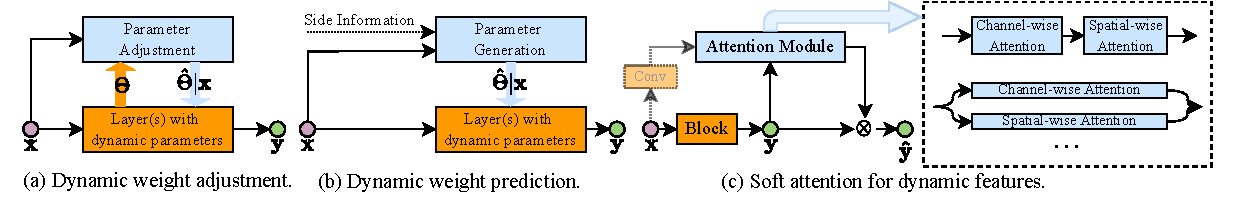
\includegraphics[width=0.9\linewidth]{6_dynamic_parameter.pdf}
    \vskip -0.2in
    \caption{{Three implementations of dynamic parameters: adjusting (a) or generating (b) the backbone parameters based on the input, and (c) dynamically rescaling the features with the attention mechanism.}}
    \label{dynamic_params}
    \vskip -0.2in
\end{figure*}


\vspace{-1.5ex}
\subsection{Dynamic Parameters} \label{adaptive_params}
\vspace{-0.25ex}
Although the networks with dynamic \emph{architectures} in Sec. \ref{dynamic_arch} can adapt their inference graphs to each sample and achieve an efficient allocation of computation, they usually have special architecture designs, requiring specific training strategies or careful hyper-parameters tuning (Sec. \ref{sec:discussion}).
% , which might limit their applicability to some extent. 

Another line of work adapts network \emph{parameters} to different inputs while keeping the architectures fixed, which has been shown effective in improving the representation power of networks with a minor increase of computational cost. Given an input sample $\mathbf{x}$, 
% if we denote a function (a network or a layer in the network) parameterized by $\bm{\Theta}$ as $\mathcal{F}(\cdot,\bm{\Theta})$, 
the output of a conventional network (module) with static parameters can be written as $\mathbf{y}\! =\!\mathcal{F}(\mathbf{x},\bm{\Theta})$. In contrast, the output of a model with dynamic parameters could be represented by
% \vskip -0.1in
\begin{equation}
  \setlength{\abovedisplayskip}{3pt}
  \mathbf{y} = \mathcal{F}(\mathbf{x},\bm{\hat{\Theta}}|\mathbf{x}) = \mathcal{F}(\mathbf{x},\mathcal{W}(\mathbf{x}, \bm{\Theta})),
  \label{eq:dynamic_parameter}
  \setlength{\belowdisplayskip}{3pt}
\end{equation}
% \vskip -0.1in
where $\mathcal{W}(\cdot, \bm{\Theta})$ is the operation producing input-dependent parameters, and its design has been extensively explored.

In general, the parameter adaptation can be achieved from three aspects (see \figurename~\ref{dynamic_params}): 1) adjusting the trained parameters based on the input (Sec. \ref{dynamic_param_adjust}); 2) directly generating the network parameters from the input (Sec. \ref{weight_predict}); and 3) rescaling the features with soft attention (Sec. \ref{sec:attention}).

\vspace{-1ex}
\subsubsection{Parameter Adjustment}
\label{dynamic_param_adjust}
\vspace{-0.5ex}
A typical approach to parameter adaptation is adjusting the weights based on their input during inference as presented in \figurename~\ref{dynamic_params} (a). This implementation usually evokes little computation to obtain the adjustments, e.g., attention weights \cite{harley_segmentation-aware_2017, su_pixel-adaptive_2019,yang2019condconv,chen_dynamic_2020_attentionOver} or sampling offsets \cite{dai2017deformable,zhu_deformable_2019,gao_deformable_2019}.

\noindent\textbf{1) Attention on weights.} {To improve the representation power without noticeably increasing the computation, 
% e.g. conditionally parameterized convolution (CondConv) \cite{yang2019condconv} and dynamic convolutional neural network (DY-CNN) \cite{chen_dynamic_2020_attentionOver}, 
soft attention can be performed on multiple convolutional kernels, producing an adaptive ensemble of parameters \cite{yang2019condconv,chen_dynamic_2020_attentionOver}.}
% which has been shown more effective than simply setting a larger channel number at each layer. 
Assuming that there are $N$ kernels $\mathbf{W}_n, n\! =1,2,\!\cdots\!,N$, such a dynamic convolution 
% \footnote{For simplicity, the bias in convolution, Batch Normalization and activation functions are omitted here.} 
can be formulated as 
\begin{equation}
  \setlength{\abovedisplayskip}{3pt}
\mathbf{y} = \mathbf{x} \star \mathbf{\tilde{W}} = \mathbf{x} \star (\sum\nolimits_{n=1}^N \alpha_n\mathbf{W}_n). 
\setlength{\belowdisplayskip}{3pt}
\end{equation}
This procedure increases the model capacity yet remains high efficiency, as the result obtained through fusing the outputs of $N$ convolutional branches (as in MoE structures, see \figurename~\ref{multi_branch} (a)) is equivalent to that produced by performing once convolution with $\mathbf{\tilde{W}}$. However, only $\sim\!1/N$ times of computation is consumed in the latter approach.
% \vskip -0.1in
% \begin{equation}
 
% \end{equation}
% \vskip -0.05in

% Different from CondConv \cite{yang2019condconv} that adopts sigmoid to scale the attention weights, \emph{SoftMax} is utilized in DY-CNN \cite{chen_dynamic_2020_attentionOver} to generate normalized weight values.
% Moreover, such approach is also exploited in \cite{cheng_real-time_2020} for human activity recognition.

Weight adjustment could also be achieved by performing soft attention over the \emph{spatial locations} of convolutional weights \cite{harley_segmentation-aware_2017, su_pixel-adaptive_2019}. For example, segmentation-aware convolutional network \cite{harley_segmentation-aware_2017} applies locally masked convolution to aggregate information with larger weights from similar pixels, which are more likely to belong to the same object.
% , and the similarity is estimated according to the distance between pixel embeddings.
Unlike \cite{harley_segmentation-aware_2017} that requires a sub-network for feature embedding, pixel-adaptive convolution (PAC) \cite{su_pixel-adaptive_2019} adapts the convolutional weights based on the attention mask generated from the input feature at each layer.

{Instead of adjusting weights conditioned on every sample itself, meta-neighborhoods \cite{shan2020meta} adapt the network parameters to each input sample based on its similarity to the neighbors stored in a dictionary.}

\noindent\textbf{2) Kernel shape adaptation.} 
% To recognize objects of varying scales and shapes, 
Apart from adaptively scaling the weight \emph{values}, parameter adjustment can also be realized to reshape the convolutional kernels and achieve \emph{dynamic reception of fields}. Towards this direction, 
% numerous research efforts are made to learn feature-dependent offsets for convolutional kernels. Specifically, 
deformable convolutions \cite{dai2017deformable,zhu_deformable_2019} sample feature pixels from adaptive locations when performing convolution on each pixel. Deformable kernels \cite{gao_deformable_2019} samples weights in the kernel space to adapt the \emph{effective} reception field (ERF) while leaving the reception field unchanged. Table \ref{tab:deform_kernels} summarizes the formulations of the above three methods. 
% Note that the main difference between \cite{dai2017deformable} and \cite{zhu_deformable_2019} is that the latter version introduces a dynamic spatial-wise modulation mechanism.
%  These kernel shape adaptation approaches all lead to significant improvements in accuracy on image classification and object detection tasks. 
{Due to their irregular memory access and computation pattern, these kernel shape adaptation approaches typically require customized CUDA kernels for the implementation on GPUs. However, recent literature has shown that the practical efficiency of deformable convolution could be effectively improved by co-designing algorithm and hardware based on embedded devices such as FPGAs \cite{huang2021codenet}.}
% Different to regular convolutions which process a fixed grid of pixels, the dynamic operation may access arbitrary feature pixels, and thus customized CUDA kernels are required for implementation on GPU \cite{dai2017deformable,zhu_deformable_2019}. 
% Instead of learning entirely free offsets as in \cite{dai2017deformable,zhu_deformable_2019,gao_deformable_2019}, local receptive adaptation \cite{shelhamer_blurring_2019} combines free-form filters and structured gaussian filters parameterized by data-dependent covariance matrices, and dynamically rescales the learned free-form filters by convolving them with the structured gaussian filters.
% Wang et al. \cite{wang_dynamic_2019} further develop the method in \cite{shelhamer_blurring_2019} by tuning the models via optimizing the structure parameter learning for $\Sigma$.
\begin{table*}
  \vspace{-2ex}
  \caption{{Kernel shape adaptation by dynamically sampling feature pixels \cite{dai2017deformable,zhu_deformable_2019} or convolutional weights \cite{gao_deformable_2019}.}}
  \vspace{-4ex}
  \label{tab:deform_kernels}
  \begin{center}
    \begin{tabular}{c|c|c|c}
      \hline
      \textbf{Method} & \textbf{Formulation} & \textbf{Sampled Target} & \textbf{Dynamic Mask} \\
      \hline
      Regular Convolution & $\mathbf{y(p)} = \sum\nolimits_{k=1}^K \mathbf{W}(\mathbf{p}_k) \mathbf{x}(\mathbf{p+p}_k)$ & - & -  \\
      \hline
      Deformable ConvNet-v1 \cite{dai2017deformable} & $\mathbf{y(p)} = \sum\nolimits_{k=1}^K \mathbf{W}(\mathbf{p}_k) \mathbf{x}(\mathbf{p+p}_k+\Delta \mathbf{p}_k)$ & Feature map & No  \\
      Deformable ConvNet-v2 \cite{zhu_deformable_2019} & $\mathbf{y(p)} = \sum\nolimits_{k=1}^K \mathbf{W}(\mathbf{p}_k) \mathbf{x}(\mathbf{p+p}_k+\Delta \mathbf{p}_k)\Delta \mathbf{m}_k$ & Feature map & Yes  \\
      Deformable Kernels \cite{gao_deformable_2019} & $\mathbf{y(p)} = \sum\nolimits_{k=1}^K \mathbf{W}(\mathbf{p}_k+\Delta \mathbf{p}_k) \mathbf{x}(\mathbf{p+p}_k)$ & Conv kernel & No \\
      \hline
    \end{tabular}
  \end{center}
  \vspace{-5ex}
\end{table*}

\vspace{-1ex}
\subsubsection{Weight Prediction} \label{weight_predict}
\vspace{-0.25ex}
% Different to the weight adjustment paradigm introduced in Sec. \ref{dynamic_param_adjust} that 
Compared to making modifications on model parameters on the fly (Sec. \ref{dynamic_param_adjust}), weight prediction \cite{denil_predicting_2013} is more straightforward: it directly generates (a subset of) input-adaptive parameters with an independent model at test time (see \figurename~\ref{dynamic_params} (b)). This idea was first suggested in \cite{schmidhuber1992learning}, where both the weight prediction model and the backbone model were feedforward networks. Recent work has further extended the paradigm to modern network architectures and tasks.
% which has been applied at the \emph{training} stage to generate static models for specific tasks \cite{denil_predicting_2013,von_oswald_continual_2019}.
% for years in various fields including learning to learn \cite{wang_learning_2016} and continual learning \cite{von_oswald_continual_2019}, etc. 
% A type of dynamic networks realize weight prediction to process each instance with content-aware parameters during \emph{inference}. 
% Note that the idea of using a separate network to produce context-dependent weight changes for the other one at test time was suggested in \cite{schmidhuber1992learning}, where both models were feedforward networks. Recent work implements this idea on modern network architectures, and a variety of researches have generalized the scheme on different tasks.
% Here we first introduce several general network designs of weight prediction, and then summarize some task-specific approaches.

\noindent\textbf{1) General architectures.} Dynamic filter networks (DFN) \cite{jia2016dynamic} and HyperNetworks \cite{ha2016hypernetworks} are two classic approaches realizing runtime weight prediction for CNNs and RNNs, respectively. Specifically, a filter generation network is built in DFN \cite{jia2016dynamic} to produce the filters for a convolutional layer. As for processing sequential data (e.g. a sentence), the weight matrices of the main RNN are predicted by a smaller one at each time step conditioned on the input (e.g. a word) \cite{ha2016hypernetworks}. WeightNet \cite{ma_weightnet_2020} unifies the dynamic schemes of \cite{yang2019condconv} and \cite{hu2018squeeze} by predicting the convolutional weights via simple grouped FC layers, achieving competitive results in terms of the accuracy-FLOPs\footnote{{Floating point operations, which is widely used as a measure of inference efficiency of deep networks.}} and accuracy-parameters trade-offs.

{Rather than generating standard \emph{convolutional} weights, LambdaNetworks \cite{bello2021lambdanetworks} learns to predict the weights of \emph{linear} projections based on the contexts of each pixel together with the relative position embeddings, showing advantages in terms of computational cost and memory footprint.}

% Moreover, weight prediction can also be applied to achieve \emph{spatial-wise} dynamic parameters by generating location-specific filters \cite{jia2016dynamic,wu_dynamic_2018,wang_carafe_2019,chen_dynamic_2020}, which will be further discussed in Sec. \ref{sec_spatially_adaptive}.


\noindent\textbf{2) Task-specific information} 
% In addition to regular features, 
has also been exploited to predict model parameters on the fly, enabling dynamic networks to generate task-aware feature embeddings. For example, edge attributes are utilized in \cite{simonovsky_dynamic_2017} to generate filters for graph convolution, and camera perspective is incorporated in \cite{kang2017incorporating} to generate weights for image convolution. {Such task-aware weight prediction has been shown effective in improving the data efficiency on many tasks, including visual question answering \cite{de2017modulating,perez2018film} and few-shot learning \cite{bertinetto2016learning,wang2019tafe}.}



\vspace{-1ex}
\subsubsection{Dynamic Features} \label{sec:attention}
\vspace{-0.25ex}
The main goal of either \emph{adjusting} (Sec. \ref{dynamic_param_adjust}) or \emph{predicting} (Sec. \ref{weight_predict}) model parameters is producing more dynamic and informative features, and therefore enhancing the representation power of deep networks. A more straightforward solution is rescaling the features with input-dependent soft attention (see \figurename~\ref{dynamic_params} (c)), which requires minor modifications on computational graphs. Note that for a linear transformation $\mathcal{F}$, applying attention $\bm{\alpha}$ on the output is equivalent to performing computation with re-weighted parameters, i.e.
\begin{equation}\label{dynamic_feature_key}
  \setlength{\abovedisplayskip}{3pt}
    \mathcal{F}(\mathbf{x},\bm{\Theta})\otimes \bm{\alpha}= \mathcal{F}(\mathbf{x},\bm{\Theta}\otimes\bm{\alpha}).
    \setlength{\belowdisplayskip}{3pt}
\end{equation}
% \vskip -0.05in

% origins in \cite{vaswani2017attention} for learning long dependencies of texts, and 
% further extended to CV tasks by Non-local networks \cite{wang2018non} and some other variants \cite{yue2018compact,huang2019ccnet}. 
% \cite{chen20182,yue2018compact,fu2019dual,huang2019ccnet}. 
% To put it simply, self attention is developed to 
% Specially, we take channel-wise attention as an example to demonstrate that such attention mechanism can be equivalent to performing convolution with adaptive weights as those dynamic operations mentioned in the previous subsections.

% \begin{figure}
%   \centering
%   % \vspace{-1ex}
%     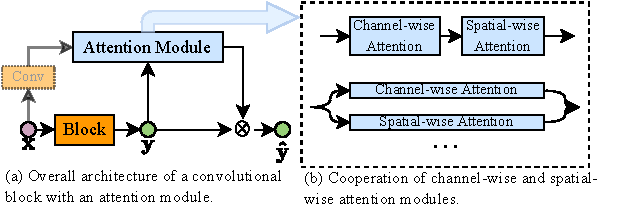
\includegraphics[width=\linewidth]{7_soft_attention.pdf}
%     \vskip -0.1in
%     \caption{Soft attention mechanism for dynamic features.}
%     \label{dynamic_recalibration}
%     \vspace{-3ex}
% \end{figure}
% The dashed arrows and module denote an optional inference path, which means that the attention is generated based on the input feature of the block
\noindent\textbf{1) Channel-wise attention} is one of the most common soft attention mechanisms. Existing work typically follows 
% , and extensive approaches to generating effective attentional weights have been studied. 
% Most researches follow 
the form in squeeze-and-excitation network (SENet) \cite{hu2018squeeze}:
\begin{equation}\label{se_attention}
  \setlength{\abovedisplayskip}{3pt}
\mathbf{\tilde{y}}\! = \!\mathbf{y} \otimes \bm{\alpha}\! =\!\mathbf{y} \otimes \mathcal{A}(\mathbf{y}),  \bm{\alpha}\in\left[0,1\right]^C.
\setlength{\belowdisplayskip}{3pt}
\end{equation} 
In Eq. \ref{se_attention}, $\mathbf{y}\! =\!\mathbf{x} \star \mathbf{W}$ is the output feature of a convolutional layer with $C$ channels, and $\mathcal{A}(\cdot)$ is a lightweight function composed of pooling and linear layers for producing $\bm{\alpha}$.
% which exploits pooling and linear layers to produce channel-wise attention for the output feature of a convolution layer. 
% This procedure can be represented by $\mathbf{\tilde{y}}\! = \!\mathbf{y} \otimes \bm{\alpha},$
% \begin{equation}
%   \mathbf{\tilde{y}} = \mathbf{y} \otimes \bm{\alpha} = \mathbf{y} \otimes \sigma(\mathrm{FC}_2(\mathrm{ReLU}(\mathrm{FC}_1(\mathrm{GAP}(\mathbf{y}))))),
% \end{equation}
% where $\bm{\alpha}\!\in\!\mathbb{R}^C$ is the attention generated from $\mathbf{y}$, and $C$ is the number of channels. 
Taking the convolution into account, the procedure can also be written as $\mathbf{\tilde{y}}\! = \!(\mathbf{x} \star \mathbf{W}) \otimes \bm{\alpha}\! =\! \mathbf{x} \star (\mathbf{W} \otimes \bm{\alpha})$, from which we can observe that applying attention on features is equivalent to performing convolution with dynamic weights.
% As mentioned in Sec. \ref{weight_predict}, such equivalent is exploited by \cite{ma_weightnet_2020}, which unifies the two computational paradigms in one framework, and directly \emph{generates} convolutional weights.

% discover that performing attention on convolutional weights (e.g. CondConv \cite{yang2019condconv} in Sec. \ref{dynamic_param_adjust}) and on feature channels (e.g. SENet \cite{hu2018squeeze}) can be unified in one framework, and further propose WeightNet \cite{ma_weightnet_2020}, 

Other implementations for attention modules have also been developed, including using standard deviation to provide more statistics \cite{lee2019srm}, or replacing FC layers with efficient 1D convolutions \cite{wang_eca-net_2020}.
% , which can also avoid the squeeze operation in \cite{hu2018squeeze} that may have side effect on capturing dependencies across all channels. 
% For instance, apart from average pooling utilized in \cite{hu2018squeeze}, standard deviation of features is exploited for attention generation in \cite{lee2019srm}. Instead of stacking FC layers, ECA-Net \cite{wang_eca-net_2020} adopts 1D convolution, which is more efficient, and can avoid the squeeze operation in \cite{hu2018squeeze} that may have side effect on capturing dependencies across all channels. 
The empirical performance of three computational graphs for soft attention is studied in \cite{guo_spanet_2020}: 1) $\mathbf{\tilde{y}}\! =\!\mathbf{y}\otimes \mathcal{A}(\mathbf{y})$, 2) $\mathbf{\tilde{y}}\! =\!\mathbf{y}\otimes \mathcal{A}(\mathbf{x})$ and 3) $\mathbf{\tilde{y}}\! =\!\mathbf{y}\otimes \mathcal{A}(\mathrm{Conv}(\mathbf{x}))$. It is found that the three forms yield different performance in different backbone networks.

% \cite{ma2020activate} first proposes a family of activation functions parameterized by $\beta$, and further adopts an SE-like module to predict $\beta$ from the input on the fly.
% Competitive SENet \cite{hu2018competitive} take the input and output of a residual block and apply SE-like modules on them, generating the attention for the output by fusing the global information from both the input and output features. Style-based Recalibration Module (SRM) \cite{lee2019srm} utilizes a global AvgPool (average pooling) and a global StdPool (standard deviation pooling) to represent the style information for each channel of the input, and further adopts a sequence of FC layer, BN, Sigmoid function to obtain the channel-wise attention. Wang et al. \cite{wang_eca-net_2020} achieve channel attention by performing 1D convolution on the $c$-dimensional tensor generate by the GAP operation, reducing the parameters of FC layers and meanwhile avoiding the squeeze procedure in SE Modules. On the task of semantic segmentation, Zhang et al. \cite{zhong_squeeze-and-attention_2020} directly generate the attention for the output with input features, and replacing the identical feature in the skip connection with the attention tensor. Instead of performing one GAP operation, SPANet \cite{guo_spanet_2020} sets three adaptive pooling branches, downsampling the input to the size of $4\times 4, 2\times 2, 1\times 1$ respectively. The multi-branch pooing output is further fused and concatenated, fed into MLPs to generate the channel-wise attention. If we denote $\mathcal{A}(\cdot)$ as the attention module composed of pooling layers, convolutional layers and MLPs, and $\mathbf{x}$ is the input feature, $\mathbf{y, \tilde{y}}$ are the output tensor before and after recalibration with attention, the attention paths in \cite{guo_spanet_2020} can be summarized into three types (see \figurename~\ref{dynamic_recalibration} (a)): 1) $\mathbf{\tilde{y}}=\mathbf{y}\otimes \mathcal{A}(\mathbf{y})$; 2) $\mathbf{\tilde{y}}=\mathbf{y}\otimes \mathcal{A}(\mathbf{x})$; 3) $\mathbf{\tilde{y}}=\mathbf{y}\otimes \mathcal{A}(\mathrm{Conv}_0(\mathbf{x}))$. Dynamic ReLU \cite{chen_dynamic_2020_relu} achieves dynamic channel-wise attention by replacing the static ReLU activation function for each feature channel ($\mathbf{y}_c = \max (\mathbf{x}_c, 0)$) with the max value among $K$ linear transformations of the feature channel $\mathbf{y}_c = \max_{1\le k\le K} \left\{a_c^k \mathbf{x}_c + b_c^k\right\}$, where $c$ is the channel index and $a_c^k, b_c^k$ are linear coefficients learned by a SE-like structure conditioned on the input $\mathbf{x}$.

\noindent\textbf{2) Spatial-wise attention}. Spatial locations in features could also be dynamically rescaled with attention to improve the representation power of deep models \cite{wang2017residual}. Instead of using pooling operations to efficiently gather global information as in channel-wise attention, convolutions are often adopted in spatial-wise attention to encode local information. Moreover, these two types of attention modules can be integrated in one framework \cite{roy2018concurrent,chen_sca-cnn_2017, woo_cbam_2018,hu2018gather} (see \figurename~\ref{dynamic_params} (c)).
% or be generated from and applied on multiple channels \cite{hu2018gather}/channel groups \cite{li_spatial_2019} independently.
% by 1) building parallel attention modules \cite{roy2018concurrent}; or 2) applying them sequentially \cite{chen_sca-cnn_2017, woo_cbam_2018}, or 3) 
% directly generate spatial-wise attention maps dependent on 
% Concurrent Spatial and Channel Squeeze-and-Excitation (scSE) is proposed in \cite{roy2018concurrent} to perform spatial \& channel attention respectively in fully convolutional networks \cite{ronneberger2015u, jegou2017one} for semantic segmentation. The channel attention in \cite{roy2018concurrent} is implemented by an SE module, and the spatial attention is achieved via a similar procedure: a $1\!\times\! 1$ convolution layer transforms the feature to the size of $h\!\times\! w\!\times\! 1$, and after scaled by a sigmoid function, the attention is multiplied with the original feature. The output of the two attention branches are combined via summation. BAM \cite{park_bam_2018} builds the channel attention module and spatial attention model in a parallel structure, and the two branches of scaling factors are first added before conducting element-wise multiplication with the input features. Moreover, the spatial attention module is implemented as a sequence of convolutional layers in \cite{park_bam_2018}. On the task of image caption, SCA-CNN \cite{chen_sca-cnn_2017} makes use of hidden units in the LSTM together with intermediate feature maps in the CNN and apply linear transformations on them to generate channel-wise attention and spatial-wise attention consecutively. CBAM \cite{woo_cbam_2018} applies channel attention and spatial attention modules in a cascaded way, and for both the modules, MaxPool (max pooling) together with AvgPool are used to aggregate the global information. For the spatial attention, different to scSE, CBAM first performs the two pooling methods on the input feature along the channel dimension, and then concatenates the two pooled tensor. Finally, a $7\!\times\! 7$ convolution is conducted on the $h\!\times\! w\!\times\!2$ tensor to generate the spatial attention. Instead of applying two independent attention modules, some other methods generate the spatial attention masks for different channels/groups of channels. Residual Attention Network \cite{wang2017residual} adopts a bottleneck-shaped multi-layer branch to generate a soft mask over the output feature.
% Spatial Group-wise Enhance (SGE) \cite{li_spatial_2019} recalibrates the $g$-th group of feature $\mathbf{x}_g$ with a spatial-wise attention mask, and the procedure can be represented by
% \begin{equation}
%   \mathbf{\tilde{x}}_g = \mathbf{x}_g \otimes \sigma(\mathrm{BN}(\mathbf{x}_g\otimes\mathrm{GAP}(\mathbf{x}_g))).
% \end{equation}
% Gather-and-Excitation Network (GENet) \cite{hu2018gather} first gathers the spatial information within a reception field for each input channel by average pooling (parameter-free, GE-$\theta^-$) or depth-wise convolutions (parameterized, GE-$\theta$), and then upsample the gathered tensor to the original feature size as the attention map. Recall that SENet \cite{hu2018squeeze} adopts the parameter-free GAP operation for feature gathering while using a two-layer sub-network for parameterized feature excitation, GE-$\theta^+$ is implemented with both the gathering and excitation operations being parameterized.

\noindent\textbf{3) Dynamic activation functions.} The aforementioned approaches to generating dynamic features usually apply soft attention before static activation functions. A recent line of work has sought to increase the representation power of models with dynamic activation functions \cite{chen_dynamic_2020_relu,ma2020funnel}. For instance, 
% FReLU \cite{ma2020funnel} replaces the linear transformation in PReLU ($y\! =\!\max (x, px)$) with a 2D convolution ($y\! =\!\max (x,\mathcal{T}(x))$). 
DY-ReLU \cite{chen_dynamic_2020_relu} replaces ReLU $(\mathbf{y}_c\! =\!\max (\mathbf{x}_c, 0))$ with the max value among $N$ linear transformations $\mathbf{y}_c\! =\!\max_{n} \left\{a_c^n \mathbf{x}_c + b_c^n\right\}$, where $c$ is the channel index, and $a_c^n, b_c^n$ are linear coefficients calculated from $\mathbf{x}$. On many vision tasks, these dynamic activation functions can effectively improve the performance of different network architectures with negligible computational overhead.

To summarize, soft attention has been exploited in many fields due to its simplicity and effectiveness. Moreover, it can be incorporated with other methods conveniently. E.g., by replacing the weighting scalar $\alpha_n$ in Eq. \ref{eq_moe} with channel-wise \cite{li_selective_2019} or spatial-wise \cite{wang_autoscaler_2016} attention, the output of multiple branches with independent kernel sizes \cite{li_selective_2019} or feature resolutions \cite{wang_autoscaler_2016} are adaptively fused.
% the attention mechanism can be utilized  to dynamically fuse  . 

Note that we leave out the detailed discussion on the self attention mechanism, which is widely studied in both NLP \cite{vaswani2017attention, devlin_bert_2019} and CV fields \cite{wang2018non,yue2018compact,dosovitskiy2020image} to re-weight features based on the similarity between queries and keys at different locations (temporal or spatial). 
Readers who are interested in this topic may refer to review studies \cite{chaudhari2019attentive,zhu2019empirical,khan2021transformers}. In this survey, we mainly focus on the feature re-weighting scheme in the framework of dynamic inference. 

\vspace{-2ex}
\section{Spatial-wise Dynamic Networks}
\vspace{-0.25ex}
\label{sec_spatially_adaptive}
In visual learning, it has been found that not all locations contribute equally to the final prediction of CNNs \cite{zhou2016learning}, which suggests that \emph{spatially} dynamic computation has great potential for reducing computational redundancy.
% reveals the widely existing spatial redundancy. 
% It is natural to believe that 
In other words, making a correct prediction may only require processing a fraction of pixels or regions with an adaptive amount of computation. Moreover, based on the observations that low-resolution representations are sufficient to yield decent performance for most inputs \cite{howard2017mobilenets}, the static CNNs that take in all the input with the same resolution may also induce considerable redundancy.

To this end, spatial-wise dynamic networks are built to perform adaptive inference with respect to different spatial locations of images.
% treat different spatial locations of each input image in data-dependent manners, leading to finer-grained adaptive inference. 
According to the granularity of dynamic computation, we further categorize the relevant approaches into three levels: {\emph{pixel level} (Sec. \ref{pixel_level}), \emph{region level} (Sec. \ref{region_level}) and \emph{resolution level} (Sec. \ref{dynamic_resolution}).}

% According to the granularity of dynamic computation, we further categorize the relevant approaches into three levels: 1) \emph{pixel level}, where each pixel is treated dynamically (Sec. \ref{pixel_level}); 2) \emph{region level}, where a continuous region/patch is attended to by the model (Sec. \ref{region_level}); and 3) \emph{resolution level}, where each input image is processed with adaptive resolutions (Sec. \ref{dynamic_resolution}).

% the model only attends to strategically selected regions 
% Moreover, based on the observations that low-resolution representations are sufficient for models to yield descent error \cite{howard2017mobilenets}, another line of work exploits the redundancy in high-resolution representations, and proposes to dynamically adjust the \emph{resolution} of features at test time (Sec. \ref{dynamic_resolution}). 
% In the following subsections, we introduce these three categories of approaches respectively.

\vspace{-2ex}
\subsection{Pixel-level Dynamic Networks}
\vspace{-0.25ex}
\label{pixel_level}
% The finest-grained spatial-wise dynamic networks treats diffe spatial locations in features at the pixel level differently during inference. 
% Unlike common CNNs that apply uniform operations for each position in features, a type of 
Commonly seen spatial-wise dynamic networks perform adaptive computation at the pixel level. Similar to the categorization in Sec. \ref{sec_sample_wise}, pixel-level dynamic networks are grouped into two types: models with pixel-specific \emph{dynamic architectures}  (Sec. \ref{pixel_dynamic_arch}) and \emph{dynamic parameters} (Sec. \ref{pixel_dynamic_param}).

% 1) models with \emph{dynamic architectures} that adapt their depth or width to each feature pixel (Sec. \ref{pixel_dynamic_arch}); 2) networks with \emph{dynamic parameters} that perform convolutions with pixel-specific weights for improved flexibility of feature representation (Sec. \ref{pixel_dynamic_param}).

% where certain modules (e.g. layers or channels) are adaptively activated for a subset of pixels. Moreover, in each layer, \emph{dynamic convolution} (Sec. \ref{pixel_dynamic_conv}) can be implemented by 1) only performing the convolution on selected locations \cite{ren_sbnet_2018,xie_spatially_2020} to save the redundant computation; 2) conducting convolution with pixel-specific kernels \cite{chen_dynamic_2020,dai2017deformable,wang_adaptively_2019} for more abundant feature encoding; or 3) directly applying pixel-wise attention \cite{woo_cbam_2018} to adaptively rescale different feature locations, which is easier to realize compared to the other two approaches. 

% Unlike common CNNs that apply uniform operations for each position of features, a type of dynamic networks are designed to process every pixel with \emph{dynamic architectures} \cite{figurnov2017spatially,li_not_2017,kirillov2020pointrend} (Sec. \ref{pixel_sub_network}), where certain modules (e.g. layers or channels) are adaptively activated for a subset of pixels. Moreover, in each layer, \emph{dynamic convolution} (Sec. \ref{pixel_dynamic_conv}) can be implemented by 1) only performing the convolution on selected locations \cite{ren_sbnet_2018,xie_spatially_2020} to save the redundant computation; 2) conducting convolution with pixel-specific kernels \cite{chen_dynamic_2020,dai2017deformable,wang_adaptively_2019} for more abundant feature encoding; or 3) directly applying pixel-wise attention \cite{woo_cbam_2018} to adaptively rescale different feature locations, which is easier to realize compared to the other two approaches. 


% In the following paragraphs, we will introduce these approaches respectively. 

%  or parameters \cite{bhowmik_training-free_2017,jo_deep_2018,roy2018concurrent,chen_sca-cnn_2017,woo_cbam_2018,hu_meta-sr_2019,wang_carafe_2019,sun_learned_2020,chen_dynamic_2020} at a pixel-level, and others only performs the convolution operation on those strategically selected positions \cite{dong_more_2017,ren_sbnet_2018,cao_seernet_2019,kong_pixel-wise_2019,xie_spatially_2020,verelst_dynamic_2020}, or breaks the conventional rules of convolution to achieve adaptive reception fields for each input pixel \cite{dai2017deformable, zhu_deformable_2019,wang_adaptively_2019,gao_deformable_2019}.
\vspace{-1ex}
\subsubsection{Pixel-wise Dynamic Architectures} \label{pixel_dynamic_arch}
\vspace{-0.25ex}
Based on the common belief that foreground pixels are more informative and computational demanding than those in the background, some dynamic networks learn to adjust their architectures for each pixel. Existing literature generally achieves this by 1) \emph{dynamic sparse convolution}, which only performs convolutions on a subset of sampled pixels; 2) \emph{additional refinement}, which strategically allocates extra computation (e.g. layers or channels) on certain spatial positions.


\begin{figure}
  \centering
  \vspace{-1ex}
    \includegraphics[width=\linewidth]{8_spatial_pixel_sparse.pdf}
    \vskip -0.15in
    \caption{{Dynamic convolution on selected spatial locations. The 1 elements (black) in the spatial mask determine the pixels (green) that require computation in the output feature map.}}
    \label{fig_spatial_location_specific}
    \vspace{-3ex}
\end{figure}
\noindent\textbf{1) Dynamic sparse convolution.} To reduce the unnecessary computation on less informative locations, convolution can be performed only on strategically sampled pixels. Existing sampling strategies include 1) making use of the intrinsic sparsity of the input \cite{ren_sbnet_2018}; 2) predicting the positions of zero elements on the output \cite{dong_more_2017,cao_seernet_2019}; and 3) estimating the saliency of pixels \cite{kong_pixel-wise_2019,verelst_dynamic_2020,xie_spatially_2020}. A typical approach is using an extra branch to generate a spatial mask, determining the execution of convolution on each pixel (see \figurename~\ref{fig_spatial_location_specific}). {Pixel-wise dynamic depth could also be achieved based on a halting scheme \cite{figurnov2017spatially}} (see Sec. \ref{dynamic_depth}). These dynamic convolutions usually neglect the unselected positions, which might degrade the network performance. Interpolation is utilized in \cite{xie_spatially_2020} to efficiently fill those locations, therefore alleviating the aforementioned disadvantage.
% The recent stochastic feature sampling and interpolation (SFSI) \cite{xie_spatially_2020} utilizes interpolation to efficiently fill those locations, therefore alleviating the aforementioned disadvantage.
% The quality of the sampled feature locations largely determines the accuracy and efficiency of the network. 

% Different from the methods that conditionally activate \emph{network modules} on sampled pixels (Sec. \ref{pixel_sub_network}), a line of work achieves pixel-wise adaptive inference at the level of \emph{convolution}, which can be further divided into three categories: 1) selective execution of convolutions \cite{dong_more_2017,verelst_dynamic_2020,xie_spatially_2020}; 2) convolution with dynamic weights \cite{chen_dynamic_2020,dai2017deformable,gao_deformable_2019}and 3) pixel-wise attention on features \cite{chen_sca-cnn_2017,woo_cbam_2018,zhang_pixel-aware_2020}.
% The idea of performing convolution with unshared filters at different locations can be found in local convolution \cite{gregor_emergence_2010} and is widely applied on vision tasks \cite{taigman_deepface_2014,brazil_m3d-rpn_2019}, where the convolution kernels for each location are learned in the training phase and fixed during inference. Here we mainly focus on researches that process different spatial locations with dynamic parameters during inference, and discuss two forms of spatial-wise dynamic parameters which are generally equivalent yet implemented in different ways: 1) generating or modifying pixel-wise weights; 2) performing spatial-wise soft attention on features.




\noindent\textbf{2) Dynamic additional refinement.} Instead of only sampling certain pixels to perform convolutions, another line of work first conducts relatively cheap computation on the whole feature map, and adaptively activate extra modules on selected pixels for further \emph{refinement}. Representatively, dynamic capacity network \cite{almahairi2016dynamic} generates coarse features with a shallow model, and salient pixels are sampled based on the gradient information. 
% utilizes the gradient information to predict sensitive spatial locations for the network output. 
For these salient pixels, extra layers are applied to extract finer features. Similarly, specific positions are additionally processed by a fraction of convolutional filters in \cite{hua2019channel}. These methods adapt their network architectures in terms of \emph{depth} or \emph{width} at the pixel level, achieving a spatially adaptive allocation of computation.


{The aforementioned dynamic additional refinement approaches \cite{almahairi2016dynamic,hua2019channel} are mainly developed for image classification.} On the semantic segmentation task, pixel-wise \emph{early exiting} (see also Sec. \ref{dynamic_depth}) is proposed in \cite{li_not_2017}, where the pixels with high prediction confidence are output without being processed by deeper layers. PointRend \cite{kirillov2020pointrend} shares a similar idea, and applies additional FC layers on selected pixels with low prediction confidence, which are more likely to be on borders of objects. All these researches demonstrate that by exploiting the spatial redundancy in image data, dynamic computation at the pixel level beyond sample level significantly increases the model efficiency.

\vspace{-1ex}
\subsubsection{Pixel-wise Dynamic Parameters} \label{pixel_dynamic_param}
\vspace{-0.25ex}
In contrast to entirely skipping the convolution operation on a subset of pixels, dynamic networks can also apply data-dependent parameters on different pixels for improved representation power or adaptive reception fields.

\noindent\textbf{1) Dynamic weights.} {Similar to the sample-wise dynamic parameter methods (Sec. \ref{adaptive_params}), pixel-level dynamic weights are achieved by test-time \emph{adjustment} \cite{harley_segmentation-aware_2017, su_pixel-adaptive_2019}, \emph{prediction} \cite{bhowmik_training-free_2017,wu_dynamic_2018,hu_meta-sr_2019,wang_carafe_2019} or \emph{dynamic features} \cite{wang_autoscaler_2016,roy2018concurrent,chen_sca-cnn_2017,woo_cbam_2018}. Take weight prediction as an example,} typical approaches generate an $H\!\times\!W\!\times\! k^2$ kernel map to produce spatially dynamic weights ($H,W$ are the spatial size of the output feature and $k$ is the kernel size). Considering the pixels belonging to the same object may share identical weights, dynamic region-aware convolution (DRConv) \cite{chen_dynamic_2020} generates a segmentation mask for an input image, dividing it into $m$ regions, for each of which a weight generation network is responsible for producing a data-dependent kernel.
% The trained convolutional weights could be rescaled by pixel-wise attention on the fly. For example, pixel-adaptive convolution \cite{su_pixel-adaptive_2019} rescales the weights based on the distance between pairs of pixels. Apart from making dynamic modifications, \emph{weight prediction} (Sec. \ref{weight_predict}) is also adopted to directly generate location-specific convolution kernels. 

% Meanwhile, a weight generation network produces $m$ kernels, each of which is responsible for one region. 
% Compared to the methods that apply attention directly on features, the pixel-wise dynamic weight scheme may face an implementation issue.
% leading to better efficiency at the expense of a bit of kernel diversity. 

% LS-DFN \cite{wu_dynamic_2018} inherits the location-specific weight generation scheme in DFN \cite{jia2016dynamic}, and further sets a stride for sampling in a region of features rather than the fixed surrounding pixels. CARAFE \cite{wang_carafe_2019} generalizes pixel-wise weight prediction to dense prediction tasks. 
% However, predicting a kernel for each pixel can be computational expensive and unnecessary, because an area of pixels may belong to one same object and thus do not demand pixel-wise convolutional weights. Instead, DRConv \cite{chen_dynamic_2020} adopts an extra branch to generate a segmentation mask over the input feature, dividing it into $m$ regions. Meanwhile, a weight generation network produces $m$ convolutional kernels and each kernel is responsible for one region of the input.

% Instead of adopting dynamic convolution weights for different locations, SPADE \cite{park_semantic_2019} and SEAN normalization \cite{zhu_sean_2020} learn location-specific affine parameters in the normalization layers in a semantic image synthesis task. 

\noindent\textbf{2) Dynamic reception fields.} Traditional convolution operations usually have a fixed shape and size of kernels (e.g. the commonly used $3\!\times\!3$ 2D convolution). The resulting uniform reception field across all the layers may have limitations for recognizing objects with varying shapes and sizes. {To tackle this, a line of work learns to adapt the reception field for different feature pixels \cite{dai2017deformable, zhu_deformable_2019, gao_deformable_2019}, as discussed in Sec. \ref{dynamic_param_adjust}.} Instead of adapting the sampling location of features or kernels, adaptive connected network \cite{wang_adaptively_2019} realizes a dynamic trade-off among self transformation (e.g. $1\!\times\!1$ convolution), local inference (e.g. $3\!\times\!3$ convolution) and global inference (e.g. FC layer). The three branches of outputs are fused with data-dependent weighted summation. 
Besides images, the local and global information in non-Euclidean data, such as graphs, could also be adaptively aggregated.
% Active convolution unit \cite{jeon_active_2017} is a static method that learns spatially uniform offsets for each position in the convolutional kernels and exploit interpolation to sample continuous locations in features. 
% As we have introduced in Sec. \ref{dynamic_param_adjust}, the deformable convolution series \cite{dai2017deformable, zhu_deformable_2019} dynamically samples pixels from the whole feature map when performing convolutions. Moreover, an adaptive sampling can also be conducted in the kernel space rather than the feature space to achieve adaptive ERF \cite{gao_deformable_2019}.



% \noindent\textbf{3) Pixel-wise dynamic feature.} Though being equivalent to performing convolution with dynamic weights (as discussed in Sec. \ref{sec:attention}), directly applying spatial-wise soft attention on features can effectively increase the representation power of models \cite{wang_autoscaler_2016,roy2018concurrent,chen_sca-cnn_2017,woo_cbam_2018} while being easier to implement in practice.

% \subsubsection{Pixel-wise dynamic execution of network modules} \label{pixel_sub_network}
% \vspace{-0.25ex}
% Considering foreground pixels often require more expensive computation for feature encoding than those in the background, a variety of dynamic networks learn to strategically activate certain modules (e.g. layers \cite{almahairi2016dynamic,figurnov2017spatially} or channels \cite{hua2019channel}) on different spatial positions. For example, dynamic capacity network \cite{almahairi2016dynamic} performs inference with a shallow network, and then utilizes the visual attention mechanism to predict the spatial locations that the result is more sensitive to. For these locations, a deeper network is applied to obtain finer features. Similarly, specific positions selected based on an attention map is additionally processed by a fraction of convolutional filters at each layer of CGNet \cite{hua2019channel}. Moreover, as mentioned in Sec. \ref{dynamic_depth}, SACT \cite{figurnov2017spatially} executes an adaptive number of residual blocks at each pixel. These methods adapt their network architectures in terms of \emph{depth} or \emph{width} at pixel-level, 
% and have all shown effective for allocating the computation to salient positions for efficient inference.

% \vspace{-1ex}
% \subsubsection{Pixel-wise dynamic convolution} \label{pixel_dynamic_conv}
% \vspace{-0.25ex}
% Different from the methods that conditionally activate \emph{network modules} on sampled pixels (Sec. \ref{pixel_sub_network}), a line of work achieves pixel-wise adaptive inference at the level of \emph{convolution}, which can be further divided into three categories: 1) selective execution of convolutions \cite{dong_more_2017,verelst_dynamic_2020,xie_spatially_2020}; 2) convolution with dynamic weights \cite{chen_dynamic_2020,dai2017deformable,gao_deformable_2019}and 3) pixel-wise attention on features \cite{chen_sca-cnn_2017,woo_cbam_2018,zhang_pixel-aware_2020}.
% % The idea of performing convolution with unshared filters at different locations can be found in local convolution \cite{gregor_emergence_2010} and is widely applied on vision tasks \cite{taigman_deepface_2014,brazil_m3d-rpn_2019}, where the convolution kernels for each location are learned in the training phase and fixed during inference. Here we mainly focus on researches that process different spatial locations with dynamic parameters during inference, and discuss two forms of spatial-wise dynamic parameters which are generally equivalent yet implemented in different ways: 1) generating or modifying pixel-wise weights; 2) performing spatial-wise soft attention on features.
% \begin{figure}
%   \centering
%   \vspace{-2ex}
%     \includegraphics[width=\linewidth]{8_spatial_pixel_sparse.pdf}
%     \vskip -0.15in
%     \caption{Dynamic convolution on selected spatial locations.}
%     \label{fig_spatial_location_specific}
%     \vspace{-3ex}
% \end{figure}

% \noindent\textbf{1) Pixel-wise selective convolution.} To save the redundant computation at those unimportant locations, convolution can be performed only on certain pixels that are strategically sampled from the feature map.  
% % Cnvlutin \cite{albericio_cnvlutin_2016} and PredictiveNet \cite{lin_predictivenet_2017} are both hardware acceleration techniques that omit the multiplication of zero elements in the input \cite{albericio_cnvlutin_2016} or predicted zero locations in the output \cite{lin_predictivenet_2017} on the fly. 
% Existing sampling strategies include 1) making use of the sparsity of the input \cite{ren_sbnet_2018}; 2) predicting the positions of zero elements on the output \cite{dong_more_2017,cao_seernet_2019}; or 3) estimating the saliency of feature pixels \cite{kong_pixel-wise_2019,verelst_dynamic_2020,xie_spatially_2020}. Most approaches adopt an extra branch to generate a spatial mask, determining the execution of convolution on each pixel (see \figurename~\ref{fig_spatial_location_specific}), while SeerNet \cite{cao_seernet_2019} obtains the mask via once quantized inference, and only the selected pixels are computed with a full numerical precision. 

% In the aforementioned dynamic convolutions, the unselected positions are usually neglected, which may degrade the network performance. In contrast, the recent SFSI \cite{xie_spatially_2020} utilizes interpolation to fill those unselected locations with cheap computation. However, although being shown effective in reducing redundant computation, these spatial-wise sparse sampling operations can result in a gap between theoretical FLOPs reduction and runtime speedup, which will be further discussed in Sec. \ref{discuss_implement}.

% \noindent\textbf{2) Pixel-wise dynamic weights.} Instead of entirely skipping the convolution operation on a subset of pixels, another type of networks apply dynamically generated or modified convolution weights on different locations for more abundant representations or adaptive reception fields.

% a) \emph{Dynamic weight values} can be produced by modifying the trained convolutional weights with pixel-wise attention on the fly. For example, PAC \cite{su_pixel-adaptive_2019} mentioned in Sec. \ref{dynamic_param_adjust} rescales the weights by the Gaussian distance between pixel embeddings. Apart from making dynamic modifications, \emph{weight prediction} (Sec. \ref{weight_predict}) can be adopted to directly generate location-specific convolution kernels. Most approaches \cite{bhowmik_training-free_2017,wu_dynamic_2018,hu_meta-sr_2019,wang_carafe_2019} generate an $H\!\times\!W\!\times\! k^2$ kernel map where $H,W$ are the spatial size of the output feature and $k$ is the kernel size. 
% % However, predicting a kernel for each pixel can be computational expensive for neglecting semantic information of pixels. 
% Considering an area of pixels may belong to the same object and thus do not demand pixel-wise convolutional weights, DRConv \cite{chen_dynamic_2020} generates a segmentation mask over the input feature, dividing it into $m$ regions, and meanwhile, a weight generation network produces $m$ convolutional kernels, each of which is responsible for one region. Compared to the methods that apply attention directly on features, the pixel-wise dynamic weight scheme could face an implementation issue.
% % leading to better efficiency at the expense of a bit of kernel diversity. 

% % LS-DFN \cite{wu_dynamic_2018} inherits the location-specific weight generation scheme in DFN \cite{jia2016dynamic}, and further sets a stride for sampling in a region of features rather than the fixed surrounding pixels. CARAFE \cite{wang_carafe_2019} generalizes pixel-wise weight prediction to dense prediction tasks. 
% % However, predicting a kernel for each pixel can be computational expensive and unnecessary, because an area of pixels may belong to one same object and thus do not demand pixel-wise convolutional weights. Instead, DRConv \cite{chen_dynamic_2020} adopts an extra branch to generate a segmentation mask over the input feature, dividing it into $m$ regions. Meanwhile, a weight generation network produces $m$ convolutional kernels and each kernel is responsible for one region of the input.

% % Instead of adopting dynamic convolution weights for different locations, SPADE \cite{park_semantic_2019} and SEAN normalization \cite{zhu_sean_2020} learn location-specific affine parameters in the normalization layers in a semantic image synthesis task. 

% b) \emph{Dynamic reception fields.} Traditional convolution operations usually have a fixed shape and size of kernels (e.g. $3\!\times\!3$ square for 2D convolution), leading to a uniform reception field across the feature maps at each layer, which is unsuitable for recognizing objects with varying shapes and sizes. A line of work learns adaptive reception field for different positions to recognize objects with varying shapes, scales and poses. 
% % Active convolution unit \cite{jeon_active_2017} is a static method that learns spatially uniform offsets for each position in the convolutional kernels and exploit interpolation to sample continuous locations in features. 
% As introduced in Sec. \ref{dynamic_param_adjust}, the deformable ConvNet series \cite{dai2017deformable, zhu_deformable_2019} dynamically samples pixels from the whole feature map when performing convolutions, and \cite{gao_deformable_2019} samples the weights in the kernel space rather than the feature space to achieve adaptive ERF \cite{luo2016understanding}. 

% Instead of adapting the sampling location of features or kernels, adaptive connected network \cite{wang_adaptively_2019} realizes a dynamic trade-off among self transformation (e.g. $1\!\times\!1$ convolution), local inference (e.g. $3\!\times\!3$ convolution) and global inference (e.g. FC layer) by fusing the three branches of output with data-dependent weighted sum. Besides images, \cite{wang_adaptively_2019} can also be applied for aggregating the local and global information in non-Euclidean data such as graphs.

% \noindent\textbf{3) Pixel-wise dynamic feature.} As discussed in Sec. \ref{sec:attention}, applying spatial-wise soft attention on feature \cite{wang_autoscaler_2016,roy2018concurrent,chen_sca-cnn_2017,woo_cbam_2018,zhang_pixel-aware_2020} can effectively increase the representation power of models, and is equivalent to performing convolution with dynamic weights, yet easier to implement.

\vspace{-1.5ex}
\subsection{Region-level Dynamic Networks} \label{region_level}
\vspace{-0.5ex}
{Pixel-level dynamic networks mentioned in Sec. \ref{pixel_level} often require specific implementations for sparse computation, and consequently may face challenges in terms of achieving real acceleration on hardware \cite{xie_spatially_2020}.} An alternative approach is performing adaptive inference on \emph{regions/patches} of input images. There mainly exists two lines of work along this direction (see \figurename~\ref{fig_spatial_select_regions}): one performs parameterized \emph{transformations} on a region of feature maps for more accurate prediction (Sec. \ref{dynamic_transofrm}), and the other learns patch-level \emph{hard attention}, with the goal of improving the effectiveness and/or efficiency of models (Sec. \ref{hard_attention_pathces}).


\vspace{-1ex}
\subsubsection{Dynamic Transformations} \label{dynamic_transofrm}
\vspace{-0.25ex}
Dynamic transformations (e.g. affine/projective/thin plate spline transformation) can be performed on images to undo certain variations \cite{jaderberg_spatial_2015} for better generalization ability, or to exaggerate the salient regions \cite{recasens_learning_2018} for discriminative feature representation. For example, spatial transformer \cite{jaderberg_spatial_2015} adopts a localization network to generate the transformation parameters, and then applies the parameterized transformation to recover the input from the corresponding variations. 
% Furthermore, dense transformer \cite{li_dense_2017} inserts the spatial transformer layer \cite{jaderberg_spatial_2015} into an encoder-decoder network for dense prediction. 
Moreover, transformations are learned to adaptively zoom-in the salient regions on some tasks where the model performance is sensitive to a small portion of regions. 
% e.g. gaze tracking and fine-grained image classification \cite{recasens_learning_2018}.
\begin{figure}
  \centering
  \vspace{-1ex}
    \includegraphics[width=\linewidth]{9_spatial_select_regions.pdf}
    \vskip -0.15in
    \caption{{Region-level dynamic inference. The region selection module generates the transformation/localization parameters, and the subsequent network performs inference on the transformed/cropped region.}}
    \label{fig_spatial_select_regions}
    \vspace{-4ex}
\end{figure}
\vspace{-1ex}
\subsubsection{Hard Attention on Selected Patches} \label{hard_attention_pathces}
\vspace{-0.25ex}
% Since the most representative features in an image may be contained only in one small region, a type of dynamic networks directly selects and crops image patches from the input, making predictions based on these strategically selected patches. 

Inspired by the fact that informative features may only be contained in certain regions of an image, dynamic networks with hard spatial attention are explored to strategically select patches from the input for improved efficiency.
% Extensive implementations have been explored as follows.

% Several early studies formulate particular vision tasks as a sequential decision procedure \cite{itti_model_1998, butko_optimal_2009}, and the optimal searching strategies are extensively explored. 
% Recent studies have endowed modern network architectures with the behavior of adaptive patch selection. 
% adaptively select salient patches and perform inference on them. 

\noindent\textbf{1) Hard attention with RNNs.} The most typical approach is formulating a classification task as a sequential decision process, {and adopting RNNs to make iterative predictions based on selected patches \cite{mnih_recurrent_2014,li_dynamic_2017}.} For example, images are classified within a fixed number of steps, and at each step, the classifier RNN only sees a cropped patch, deciding the next attentional location until the last step is reached \cite{mnih_recurrent_2014}. An adaptive step number is further achieved by including early stopping in the action space \cite{li_dynamic_2017}. Glance-and-focus network (GFNet) \cite{wang2020glance} builds a general framework of region-level adaptive inference by sequentially focusing on a series of selected patches, and is compatible with most existing CNN architectures. The recurrent attention mechanism together with the early exiting paradigm enables both \emph{spatially} and \emph{temporally} adaptive inference \cite{li_dynamic_2017,wang2020glance}.
% The recurrent spatial attention is also applied for multi-object classification \cite{ba_multiple_2015,eslami_attend_2016} and image caption generation \cite{xu_show_2015}, e.t.c. 

% where a fixed size of patch is cropped from the original input at each time step, and \cite{xu_show_2015} uses a LSTM to generate image caption sentences word by word based on the observation on selected patches.
% In such paradigm, the localization of attention patches is essential and require specific training strategies such as RL.

\noindent\textbf{2) Hard attention with other implementations.} Rather than using an RNN to predict the region position that the model should pay attention to, class activation mapping (CAM) \cite{zhou2016learning} is leveraged in \cite{rosenfeld_visual_2016} to iteratively focus on salient patches. At each iteration, the selection is performed on the previously cropped input, leading to a progressive refinement procedure. A multi-scale CNN is built in \cite{fu_look_2017}, where the sub-network in each scale takes in the cropped patch from the previous scale, and is responsible for simultaneously producing 1) the feature representations for classification and 2) the attention map for the next scale. {Without an iterative manner, the recent differentiable patch selection \cite{cordonnier2021differentiable} adopts a differentiable top-K module to select a fixed number of patches in one step.}
% Instead of proposing only one patch at a time, \cite{xiao_application_2015,zheng_learning_2017} once proposes multiple attention patches on the fine-grained classification task. 
% and \cite{xiao_application_2015} filters out task-irrelevant patches with object-level attention. 
% For action prediction in video frames, \cite{chen_part-activated_2018} first extract features from different parts of a human body, and then selectively activate the action-related parts to enhance the representation.

\vspace{-2ex}
\subsection{Resolution-level Dynamic Networks} \label{dynamic_resolution}
\vspace{-0.5ex}
The researches discussed above typically divide feature maps into different areas (pixel-level or region-level) for adaptive inference.
% A downside of these approaches is that the sparse sampling (Sec. \ref{pixel_level}) or cropping (Sec. \ref{region_level}) operations might degrade the practical efficiency.
On a coarser granularity, some dynamic networks could treat each image as a whole by processing feature representations with adaptive resolutions. Although it has been observed that a low resolution might be sufficient for recognizing most "easy" samples \cite{howard2017mobilenets}, conventional CNNs mostly process all the inputs with the same resolution, inducing considerable redundancy. Therefore, resolution-level dynamic networks exploit spatial redundancy from the perspective of feature resolution rather than the saliency of different locations. Existing approaches mainly include 1) scaling the inputs with adaptive ratios (Sec. \ref{adaptive_scaling_ratio}); 2) selectively activating the sub-networks with different resolutions in a multi-scale architecture (Sec. \ref{dynamic_res_multiscale}).

\vspace{-1ex}
\subsubsection{Adaptive Scaling Ratios} \label{adaptive_scaling_ratio}
\vspace{-0.25ex}
Dynamic resolution can be achieved by scaling features with adaptive ratios. For example, a small sub-network is first executed to predict a scale distribution of faces on the face detection task, then the input images are adaptively zoomed, so that all the faces fall in a suitable range for recognition \cite{hao_scale-aware_2017}. A plug-in module is used by \cite{yang_dynamic-stride-net_2019} to predict the stride for the first convolution block in each ResNet stage, producing features with dynamic resolution.

\vspace{-1ex}
\subsubsection{Dynamic Resolution in Multi-scale Architectures} \label{dynamic_res_multiscale} 
\vspace{-0.25ex}
An alternative approach to achieving dynamic resolution is building multiple sub-networks in a parallel \cite{wang_elastic_2019} or cascading \cite{yang_resolution_2020} way. These sub-networks with different feature resolutions are selectively activated conditioned on the input during inference. For instance, Elastic \cite{wang_elastic_2019} realizes a \emph{soft} selection from multiple branches at every layer, where each branch performs a downsample-convolution-upsample procedure with an independent scaling ratio. To practically avoid redundant computation, a \emph{hard} selection is realized by \cite{yang_resolution_2020}, which allows each sample to conditionally activate sub-networks that process feature representations with resolution from low to high (see \figurename~\ref{multi_scale} (c) in Sec. \ref{dynamic_depth}).

\vspace{-2ex}
\begin{figure*}
  \centering
  \vspace{-2ex}
    \includegraphics[width=0.9\linewidth]{10_temporal_skim.pdf}
    \vskip -0.15in
    \caption{{Temporally adaptive inference. The first three approaches dynamically allocate computation in each step by (a) skipping the update, (b) partially updating the state, or (c) conditional computation in a hierarchical structure. The agent in (d) decides where to read in the next step.}}
    \label{fig_temporal_skim}
    \vspace{-3ex}
\end{figure*}
\section{Temporal-wise Dynamic Networks} \label{sec_temporal_adaptive}
\vspace{-0.25ex}
Apart from the spatial dimension (Sec. \ref{sec_spatially_adaptive}), adaptive computation could also be performed along the temporal dimension of sequential data, such as texts (Sec. \ref{temporal_text}) and videos (Sec. \ref{sec:tempoal_video}). {In general, network efficiency can be improved by dynamically allocating less/no computation to the inputs at unimportant temporal locations.}


% redundant computation can be generally saved from two aspects: 1) allocating cheap operations for the input at certain locations; 2) selectively conducting computation only on a subset of temporal locations.

\vspace{-1.5ex}
\subsection{RNN-based Dynamic Text Processing}
\vspace{-0.25ex}
\label{temporal_text}
Traditional RNNs mostly follow a static inference paradigm, i.e. input tokens are read sequentially to update a hidden state at each time step, which could be written as
\begin{equation}\label{eq_rnn}
  \setlength{\abovedisplayskip}{3pt}
\mathbf{h}_t = \mathcal{F}(\mathbf{x}_t, \mathbf{h}_{t-1}), t=1,2,\cdots, T.
\setlength{\belowdisplayskip}{3pt}
\end{equation}
Such a static inference paradigm induces significant redundant computation, as different tokens usually have different contributions to the downstream tasks.
% However, the multiple tokens usually have disparate contributions to the downstream tasks. 
% Therefore, the inference scheme of static RNNs could be inefficient since they process all tokens with even computation. 
A type of dynamic RNN is developed for allocating appropriate computational cost at each step. Some learn to \emph{"skim"} unimportant tokens by dynamic update of hidden states (Sec. \ref{skimming_text}), and others conduct \emph{adaptive reading} to avoid processing task-irrelevant tokens. Specifically, such adaptive reading can be achieved by \emph{early exiting} (Sec. \ref{temporal_early_exit}) or \emph{dynamic jumping} (Sec. \ref{text_jumping}).
% Note that the input token of these RNNs is free to the level of text, which could be characters \cite{graves2016adaptive}, words \cite{yu_learning_2017} or even sentences \cite{liu_finding_2020}.

\vspace{-1ex}
\subsubsection{Dynamic Update of Hidden States}
\vspace{-0.25ex}
\label{skimming_text}
Since not all the tokens are essential for capturing the task-relevant information in a sequence, dynamic RNNs can be built to adaptively update their hidden states at each time step. Less informative tokens will be coarsely \emph{skimmed}, i.e. the states are updated with cheaper computation.
% In particular, we summarize three different approaches to dynamic state updating as follows.
% by: 1) directly skipping the update \cite{campos_skip_2018,hansen_neural_2019,tao_skipping_2019}; 2) conducting a coarse update \cite{graves2016adaptive,jernite_variable_2017,seo_neural_2018}; or 3) performing selective update in hierarchical structures \cite{chung_hierarchical_2017,ke_focused_2018}.
% The three types of methods are introduced in the following paragraphs.

\noindent\textbf{1) Skipping the update.} For unimportant inputs at certain temporal locations, dynamic models can learn to entirely skip the update of hidden states (see \figurename~\ref{fig_temporal_skim} (a)), i.e.
\begin{equation}
  \setlength{\abovedisplayskip}{3pt}
  \mathbf{h}_t = \alpha_t\mathcal{F}(\mathbf{x}_t, \mathbf{h}_{t-1}) + (1-\alpha_t)\mathbf{h}_{t-1}, \alpha_t\in\left\{0,1\right\}.
  \setlength{\belowdisplayskip}{3pt}
\end{equation}
For instance, Skip-RNN \cite{campos_skip_2018} updates a controlling signal in every step to determine whether to update or \emph{copy} the hidden state from the previous step. An extra agent is adopted by Structural-Jump-LSTM \cite{hansen_neural_2019} to make the skipping decision conditioned on the previous state and the current input. Without training the RNNs and the controllers jointly as in \cite{campos_skip_2018} and \cite{hansen_neural_2019}, a predictor is trained in \cite{tao_skipping_2019} to estimate whether each input will make a "significant change" on the hidden state. The update is identified worthy to be executed only when the predicted change is greater than a threshold.

\noindent\textbf{2) Coarse update. } As directly skipping the update may be too aggressive, dynamic models could also update the hidden states with adaptively allocated operations. In specific, a network can adapt its architecture in every step, i.e.  
\begin{equation}
  \setlength{\abovedisplayskip}{3pt}
  \mathbf{h}_t = \mathcal{F}_t(\mathbf{x}_t, \mathbf{h}_{t-1}), t=1,2,\cdots, T,
  \setlength{\belowdisplayskip}{3pt}
\end{equation}
where $\mathcal{F}_t$ is determined based on the input $\mathbf{x}_t$. One implementation is selecting a subset of dimensions of the hidden state to calculate, and copying the remaining from the previous step \cite{jernite_variable_2017,seo_neural_2018}, as shown in \figurename~\ref{fig_temporal_skim} (b). To achieve the partial update, a subset of rows in weight matrices of the RNN is dynamically activated in \cite{jernite_variable_2017}, while Skim-RNN \cite{seo_neural_2018} makes a choice between two independent RNNs.

When the hidden states are generated by a multi-layer network, the update could be interrupted at an intermediate layer based on an accumulated halting score \cite{graves2016adaptive}.

To summarize, a coarse update can be realized by data-dependent network \emph{depth} \cite{graves2016adaptive} or \emph{width} \cite{jernite_variable_2017,seo_neural_2018}. 
% Let $\mathbf{h}_t[k]$ denote the $k$-th element of the state, a partial update for the first $K$ dimensions of $\mathbf{h}_t$ can be represented by 
% \begin{equation}
%   \mathbf{h}_t[k] = \left\{
%     \begin{aligned}
%     & \mathcal{F}_t(\mathbf{x}_t, h_{t-1}[k]), & k\le K, \\
%     & h_{t-1}[k], & else.
%     \end{aligned}
%     \right.
% \end{equation}


% Lugosch et al. \cite{lugosch_surprisal-triggered_2020} propose to adopt a big model depending on a surprisal-triggered mechanism, which means that an autoregressive model is adopted to predict the input for each time step based on the previous input contents and the big model is adopted to handle the input only when the autoregressor fails to predict the input.

{\noindent\textbf{3) Selective updates in hierarchical RNNs.} Considering the intrinsic hierarchical structure of texts (e.g. sentence-word-character), researchers have developed hierarchical RNNs to encode the temporal dependencies with different timescales using a dynamic update mechanism \cite{chung_hierarchical_2017,ke_focused_2018}. During inference, the RNNs at higher levels will selectively update their states conditioned on the output of low-level ones (see \figurename~\ref{fig_temporal_skim} (c)).
For example, when a character-level model in \cite{chung_hierarchical_2017} detects that the input satisfies certain conditions, it will \emph{"flush"} (reset) its states and feed them to a word-level network. Similar operations have also been realized by a gating module on question answering tasks \cite{ke_focused_2018}.}
% On question answering tasks, focused hierarchical RNN \cite{ke_focused_2018} applies a gating module to decide whether the state should be fed to the higher-level RNN (sentence-level) based on each word in the asked question.


\vspace{-1ex}
\subsubsection{Temporally Early Exiting in RNNs}
\vspace{-0.25ex}
\label{temporal_early_exit}
Despite that the dynamic RNNs in Sec. \ref{skimming_text} are able to update their states with data-dependent computational costs at each step, all the tokens still must be read, leading to inefficiency in scenarios where the task-relevant results can be obtained before reading the entire sequence.
% E.g., one could capture the main idea of a paper by reading only its title and abstract.

Ideally, an efficient model should adaptively stop reading before the last step $T$ in Eq. \ref{eq_rnn} is reached, once the captured information is satisfactory to solve the task. For instance, reasoning network (ReasoNet) \cite{shen_reasonet_2017} terminates its reading procedure when sufficient evidence has been found for question answering. 
% Once the reading stops, the last state will be fed into an answer module. 
Similarly, early stopping is implemented for sentence-level \cite{huang_length_2017} and paragraph-level \cite{liu_finding_2020} text classification, respectively. Note that the approaches discussed here focus on making early predictions with respect to the \emph{temporal} dimension of sequential input, rather than along the \emph{depth} dimension of networks as in Sec. \ref{dynamic_depth}.

\vspace{-1ex}
\subsubsection{Jumping in Texts}
\vspace{-0.25ex}
\label{text_jumping}
Although early exiting in Sec. \ref{temporal_early_exit} can largely reduce redundant computation, all the tokens must still be fed to the model one by one. More aggressively, dynamic RNNs could further learn to decide \emph{"where to read"} by strategically skipping some tokens without reading them, and directly jumping to an arbitrary temporal location (see \figurename~\ref{fig_temporal_skim} (d)).
% \begin{figure}[htbp]
%   \centering
%   \vspace{-1.5ex}
%     \includegraphics[width=\linewidth]{temporal_jump.pdf}
%     \vskip -0.2in
%     \caption{Temporal adaptive inference by dynamically jumping.}
%     \label{fig_temporal_jump}
%     \vspace{-1.5ex}
% \end{figure}

Such dynamic jumping, together with early exiting, is realized in \cite{yu_learning_2017} and \cite{yu_fast_2018}. Specifically, LSTM-Jump \cite{yu_learning_2017} implements an auxiliary unit to predict the jumping stride within a defined range, and the reading process ends when the unit outputs zero. The model in \cite{yu_fast_2018} first decides whether to stop at each step. If not, it will further choose to re-read the current input, or to skip a flexible number of words. Moreover, structural information is exploited by Structural-Jump-LSTM \cite{hansen_neural_2019}, which utilizes an agent to decide whether to jump to the next punctuation. Apart from looking ahead, LSTM-Shuttle \cite{fu_speed_2018} also allows backward jumping to supplement the missed history information.
%and the LSTM with dynamic skip connections \cite{gui_long_2019} updates its hidden state with the help of a selected history state together with the current hidden state.

\vspace{-1.5ex}
\subsection{Temporal-wise Dynamic Video Recognition}
\label{sec:tempoal_video}
\vspace{-0.25ex}
% There are numerous CV tasks involving video recognition, and 
For video recognition, where a video could be seen as a sequential input of frames, temporal-wise dynamic networks are designed to allocate adaptive computational resources for different frames. This can generally be achieved by two approaches: 1) dynamically updating the hidden states in each time step of \emph{recurrent} models (Sec. \ref{recurrent_video}), and 2) performing adaptive \emph{pre-sampling} for key frames (Sec. \ref{frame_sampling}).

% Similar to the approaches introduced in Sec. \ref{temporal_text}, RNN-based adaptive video recognition is typically realized by 1) treating unimportant frames with relatively cheap operations (a \emph{"glimpse"}) \cite{wu_liteeval_2019,vaudaux-ruth_actionspotter_2020}; 2) \emph{early exiting} \cite{fan_watching_2018,wu_dynamic_2020}; and 3) strategically decide \emph{"what to see when"} in each time step \cite{yeung_end--end_2016,su_leaving_2016,fan_watching_2018,wu_adaframe_2019}.

% The second line of work (Sec. \ref{frame_sampling}) adopts a dynamic \emph{pre-sampling} procedure for key frames (or clips, i.e. a small part of a long video) \cite{rao_attention-aware_2017,wu_multi-agent_2019,korbar_scsampler_2019}, and the subsequent computation is only performed on the selected frames/clips.
% , whose architecture is not limited to a 2D or 3D CNN.
% In this paradigm, an efficient and effective selection of frames/clips plays an important role for downstream tasks.
% Many frame selection algorithms or early prediction approaches have been explored on conventional models \cite{ryoo_human_2011,chen_dynamic_2011,amer_cost-sensitive_2012,hoai_max-margin_2012,amer_monte_2013,bhattacharya_minimally_2014,karasev_active_2014} before the emergency of deep networks.
% Similar to handling text input, the temporal-wise adaptive networks for processing video input can dynamically decide `what to see when' by key frame/clip selection or skimming/skipping unimportant frames.

\vspace{-1ex}
\subsubsection{Video Recognition with Dynamic RNNs} \label{recurrent_video}
\vspace{-0.25ex}
Video recognition is often conducted via a recurrent procedure, where the video frames are first encoded by a 2D CNN, and the obtained frame features are fed to an RNN sequentially for updating its hidden state. Similar to the approaches introduced in Sec. \ref{temporal_text}, RNN-based adaptive video recognition is typically realized by 1) treating unimportant frames with relatively cheap computation (\emph{"glimpse"}) \cite{wu_liteeval_2019,vaudaux-ruth_actionspotter_2020}; 2) \emph{early exiting} \cite{fan_watching_2018,wu_dynamic_2020}; and 3) performing dynamic \emph{jumping} to decide {"where to see"} \cite{yeung_end--end_2016,su_leaving_2016,fan_watching_2018,wu_adaframe_2019}.


% Due to the temporal redundancy in videos, task-irrelevant frames could be processed coarsely, or even be neglected, which is similar to the dynamic inference paradigm for text processing (Sec. \ref{temporal_text}).
%  which will be introduced in the following paragraphs.

\noindent\textbf{1) Dynamic update of hidden states.} To reduce redundant computation at each time step, LiteEval \cite{wu_liteeval_2019} makes a choice between two LSTMs with different computational costs. ActionSpotter \cite{vaudaux-ruth_actionspotter_2020} decides whether to update the hidden state according to each input frame. {AdaFuse \cite{meng2021adafuse} selectively reuses certain feature channels from the previous step to efficiently make use of historical information.} Recent work has also proposed to adaptively decide the numerical precision \cite{sun2021dynamic} or modalities \cite{weng2021hms,panda2021adamml} when processing the sequential input frames. Such a \emph{glimpse} procedure (i.e. allocating cheap operations to unimportant frames) is similar to the aforementioned text \emph{skimming} \cite{campos_skip_2018,hansen_neural_2019}.
% embeds frame skimming and skipping simultaneously, which means that an agent is trained to make decisions on 1) whether the current input should be used to update the hidden state; 2) which frame should be looked at next.

\noindent\textbf{2) Temporally early exiting.} Humans are able to comprehend the contents easily before watching an entire video. Such early stopping is also implemented in dynamic networks to make predictions only based on a portion of video frames \cite{fan_watching_2018,wu_dynamic_2020,ghodrati2021frameexit}. Together with the \emph{temporal} dimension, the model in \cite{wu_dynamic_2020} further achieves early exiting from the aspect of network \emph{depth} as discussed in Sec. \ref{dynamic_depth}.
% The prediction result can be output at a certain intermediate classifier, and even before the last frame is processed.
% Frame shuffle is used to produce large temporal strides and temporal forward-shift module \cite{lin2019tsm} is applied to facilitate information exchange among neighboring frames in the progressive computation strategy.

\noindent\textbf{3) Jumping in videos.} Considering encoding those unimportant frames with a CNN still requires considerable computation, a more efficient solution could be dynamically skipping some frames without watching them. Existing arts \cite{yeung_end--end_2016,su_leaving_2016,alwassel_action_2018} typically learn to predict the location that the network should jump to at each time step.
% Instead of training the jumping policy with RL as in \cite{yeung_end--end_2016,su_leaving_2016}, the policy in \cite{alwassel_action_2018} is trained with a proposed dataset containing the search sequences of human annotators. 
% for the action spotting task. 
Furthermore, both early stopping and dynamic jumping are allowed in \cite{fan_watching_2018}, where the jumping stride is limited in a discrete range.
% and an agent chooses one from the options conditioned on the input and hidden state. 
Adaptive frame (AdaFrame) \cite{wu_adaframe_2019} generates a continuous scalar within the range of $[0,1]$ as the relative location. 
% Moreover, a lightweight CNN is performed on the spatially \& temporally downsampled video to obtain the global context, which is further fed into the main LSTM to help update its states. 
% \cite{gao_listen_2020} predicts where to watch in each step at a clip level with self attention. 

\vspace{-1ex}
\subsubsection{Dynamic Key Frame Sampling} \label{frame_sampling}
\vspace{-0.25ex}
Rather than processing video frames recurrently as in Sec. \ref{recurrent_video}, another line of work first performs an adaptive \emph{pre-sampling} procedure, and then makes prediction by processing the selected subset of key frames or clips.
% Since the quality of these selected frames/clips essentially determines the efficiency and effectiveness of the network, the sampling strategies are attracting great research interests.
% Due to the wide existence of task-irrelevant information in videos, a line of work conducts video-related tasks via processing a subset of key frames/clips that are strategically selected from the input, and the quality of these selected frames/clips essentially determines the efficiency and effectiveness of a model. Note that the networks discussed here differ from the dynamic RNNs in Sec. \ref{recurrent_video} because these models first conduct an adaptive \emph{pre-sampling} procedure 

\noindent{\textbf{1) Temporal attention} is a common technique for networks to focus on salient frames.} For face recognition, neural aggregation network \cite{yang_neural_2017} uses \emph{soft} attention to adaptively aggregate frame features. To improve the inference efficiency, \emph{hard} attention is realized to remove unimportant frames iteratively with RL for efficient video face verification \cite{rao_attention-aware_2017}.
% and also used in . 

\noindent{\textbf{2) Sampling module} is also a prevalent option for dynamically selecting the key frames/clips in a video.} For example, the frames are first sampled uniformly in \cite{tang_deep_2018, wu_multi-agent_2019}, and discrete decisions are made for each selected frame to go forward or backward step by step. As for clip-level sampling, SCSample \cite{korbar_scsampler_2019} is designed based on a trained classifier to find the most informative clips for prediction. Moreover, dynamic sampling network (DSN) \cite{zheng_dynamic_2020} segments each video into multiple sections, and a sampling module with shared weights across the sections is exploited to sample one clip from each section.

 
% By simply taking the center channel of a 3D filter along its temporal dimension, a 3D convolution could be transformed into a 2D one.} 
{Adjusting multiple factors of deep models simultaneously has attracted researches in both static \cite{han2020model,fan2020rubiksnet} and dynamic networks \cite{li20202d,meng2020ar,wang2021adaptive,pan2021va}. For example, together with \emph{temporal-wise} frame sampling, \emph{spatially} adaptive computation can be achieved by spatial \cite{meng2020ar}/temporal \cite{fayyaz20213d} resolution adaptation and patch selection \cite{wang2021adaptive,verelst2021blockcopy}. It would be promising to exploit the redundancy in both \emph{input data} and \emph{network structure} for further improving the efficiency of deep networks.}

\vspace{-2ex}
\section{Inference and Training}
\label{inference_and_train}
\vspace{-0.25ex}
In previous sections, we have reviewed three different types of dynamic networks (sample-wise (Sec. \ref{sec_sample_wise}), spatial-wise (Sec. \ref{sec_spatially_adaptive}) and temporal-wise (Sec. \ref{sec_temporal_adaptive})). It can be observed that making data-dependent \emph{decisions} at the inference stage is essential to achieve high efficiency and effectiveness. Moreover, \emph{training} dynamic models is usually more challenging than optimizing static networks.

Note that since parameter adaptation (Sec. \ref{adaptive_params}) could be conveniently achieved by differentiable operations, models with dynamic parameters \cite{yang2019condconv,ma_weightnet_2020,hu2018squeeze} can be directly trained by stochastic gradient descent (SGD) without specific techniques. Therefore, in this section we mainly focus on discrete decision making (Sec. \ref{inference}) and its training strategies (Sec. \ref{training}), which are absent in most static models.
% an essential behavior of dynamic models is that they need to make data-dependent decisions during inference, and their efficiency and accuracy largely depend on these decisions. Moreover, such difference also brings training issues. 
% especially, some discrete functions are hard to be optimized due to their nondifferentiability. 
% , some of which are discrete and therefore are hard to be trained with traditional optimization methods for static models. In this section, 
% After reviewing the architecture design of dynamic networks based on their adaptive inference schemes, here 



% Here we summarize the decision making schemes (Sec. \ref{inference}) and the training strategies (Sec. \ref{training}) for dynamic DNNs. 
% with special emphasis on those making discrete decisions at test time.
\vspace{-1.5ex}
\subsection{Decision Making of Dynamic Networks}
\label{inference}
\vspace{-0.5ex}
As described above, dynamic networks are capable of making data-dependent decisions during inference to transform their architectures, parameters, or to select salient spatial/temporal locations in the input. Here we summarize three commonly seen decision making schemes as follows.


% For those models, there are some mechanisms for making decisions to control the inference graphs. Based on how these decisions are made, these adaptive models can be summarized in three different categories.
\vspace{-1ex}
\subsubsection{Confidence-based Criteria}
\vspace{-0.25ex}
Many dynamic networks \cite{teerapittayanon2016branchynet,huang2017multi,yang_resolution_2020} are able to output "easy" samples at early exits if a certain confidence-based criterion is satisfied. These methods generally require estimating the confidence of intermediate predictions, which is compared to a predefined threshold for decision making.
% and make decisions by comparing the confidence with human-defined thresholds. 
In classification tasks, the confidence is usually represented by the maximum element of the \emph{SoftMax} output \cite{huang2017multi,yang_resolution_2020}. Alternative criteria include the entropy \cite{teerapittayanon2016branchynet,xin_deebert_2020} and the score margin \cite{park2015big}. On NLP tasks, a \emph{model patience} is proposed in \cite{zhou_bert_2020}: when the predictions for one sample stay unchanged after a number of classifiers, the inference procedure stops. 
% The decision scheme in \cite{zhou_bert_2020} also resembles that in \cite{tao_skipping_2019}, which conditionally performs an update for hidden states based on how significant a change would be brought by the update. 

In addition, the halting score in \cite{graves2016adaptive,figurnov2017spatially,dehghani_universal_2019,elbayad_depth-adaptive_2020} could also be viewed as confidence for whether the current feature could be output to the next time step or calculation stage.

Empirically, the confidence-based criteria are easy to implement, and generally require no specific training techniques. A trade-off between accuracy and efficiency is controlled by manipulating the thresholds, which are usually tuned on a validation dataset. Note that the \emph{overconfidence} issue in deep models \cite{guo2017calibration,hein2019relu} might affect the effectiveness of such decision paradigm, when the incorrectly classified samples could obtain a high confidence at early exits.
\vspace{-1ex}
\subsubsection{Policy Networks} \label{inference_policy}
\vspace{-0.25ex}
It is a common option to build an additional policy network learning to adapt the network topology based on different samples. 
% a decision function for execution of multiple units in a model. 
Specifically, each input sample is first processed by the policy network, whose output directly determines which parts of the main network should be activated. For example, BlockDrop \cite{wu2018blockdrop} and GaterNet \cite{chen2019you} use a policy network to adaptively decide the \emph{depth} and \emph{width} of a backbone network. More generally, dynamic routing in a \emph{SuperNet} can also be controlled by a policy network \cite{cheng2020instanas}.
% In addition, some spatial-wise \cite{wang2020glance,wang2021adaptive} or temporal-wise \cite{wu_multi-agent_2019,zheng_dynamic_2020} \emph{sampling} methods may build an extra policy network for decision making.

One possible limitation of this scheme is that the architectures and the training process of some policy networks are developed for a specific backbone \cite{wu2018blockdrop,chen2019you}, and may not be easily adapted to different architectures. 

% It is worth noting that . This is considered as , because it can
% Moreover, these policy networks may pose challenges for the end-to-end training for making discrete decisions (see Sec. \ref{training}).
% However, popular deep models usually contain variants with multiple configurations in terms of the number of channels or stacked blocks, leading to a limitation for the applicability of this decision scheme.
%Because modern CNN families usually contain multiple variants with different configurations in terms of the number of channels or stacked blocks, researchers must re-design and re-train

\vspace{-1ex}
\subsubsection{Gating Functions} \label{inference_gating}
\vspace{-0.25ex}
% Instead of introducing an additional policy network that needs to be re-built and re-trained for different model structures (Sec. \ref{inference_policy}), a more general approach to making discrete decisions on the fly is attaching plug-in modules at arbitrary locations of a backbone network.
Gating function is a general and flexible approach to decision making in dynamic networks. It can be conveniently adopted as a plug-in module at arbitrary locations in any backbone network.
During inference, each module is responsible for controlling the local inference graph of a layer or block. The gating functions take in intermediate features and efficiently produce binary-valued gate vectors to decide: 1) which channels need to be activated \cite{lin2017runtime,gao2018dynamic, herrmann2018end,bejnordi2019batch,chen2019self} \emph{width}, 2) which layers need to be skipped \cite{veit2018convolutional,wang2018skipnet,wang_dual_2020,xia2020fully}, 3) which paths should be selected in a SuperNet \cite{li_learning_2020}, or 4) what locations of the input should be allocated computations \cite{kong_pixel-wise_2019,verelst_dynamic_2020,xie_spatially_2020, meng2021adafuse}.

Compared to the aforementioned decision policies, the gating functions demonstrate notable generality and applicability. However, due to their lack of differentiability, these gating functions usually need specific training techniques, which will be introduced in the following Sec. \ref{training}.

% \vspace{-0.5ex}
% \subsubsection{Deciding by a reinforcement learning model}
% \vspace{-0.25ex}
% Although the dynamic models in this subscetions can be categoried into previous three subscetions, we introduce them exclusively due to their sepcial implementatino, where the dynamic model is consistis of a main deep network work and an addtional reinforcement learning (RL) model. This RL model is usually used as a policy network for making discrete decision during inference. Given the input samples, such RL based policy networks can be implemented in the dynamic models for 1) selectively executing certain channels \cite{lin2017runtime} or layers \cite{wang2018skipnet}; 2) deciding the overall topology of inference graph \cite{wu2018blockdrop}; 3) controlling the early exiting of samples \cite{mcgill2017deciding}; 4) deciding the temporal location in the sequential input for subsequent time steps \cite{yeung_end--end_2016,su_leaving_2016} e.t.c.

\vspace{-2ex}
\subsection{Training of Dynamic Networks}
\vspace{-0.5ex}
\label{training}
Besides architecture design, training is also essential for dynamic networks. Here we summarize the existing training strategies for dynamic models from the perspectives of objectives and optimization.
\begin{table*}
  \scriptsize
  \vspace{-2ex}
  \caption{Applications of Dynamic Networks. For the type column, Sa, Sp and Te stand for sample-wise, spatial-wise and temporal-wise respectively.}
  \label{tab_tasks}
  \begin{center}
    \vspace{-6ex}
    \resizebox{\linewidth}{!}{
    \begin{tabular}{cccc}
      \toprule
      \textbf{Fields} & \textbf{Data} & \textbf{Type} & \textbf{Subfields \& references} \\
      \midrule
      & \multirow{6}*{\textbf{Image}} & \multirow{2}*{Sa} & Object detection (face \cite{rowley1998neural,viola_robust_2004,li_convolutional_2015}, facial point \cite{sun2013deep}, pedestrian \cite{angelova_real_time_2015}, general \cite{yang_exploit_2016,figurnov2017spatially,zhou_adaptive_2017,yang_metaanchor_2018,chen_adaptive_2019}) \\
      & & & Image segmentation \cite{tokunaga2019adaptive, li_learning_2020,wang2020deep}, Super resolution \cite{riegler_conditioned_2015}, Style transfer \cite{shen_neural_2018},  Coarse-to-fine classification \cite{jiang2020learning}\\ 
      \cmidrule{3-4}
      & &  \multirow{3}*{Sa \& Sp} & Image segmentation \cite{li_not_2017,kong_pixel-wise_2019,xie_spatially_2020,kirillov2020pointrend,wang_carafe_2019,he_dynamic_2019,wang_adaptively_2019,marin_efficient_2019,li_dense_2017,roy2018concurrent,wu_dynamicAttention_2020,zhong_squeeze-and-attention_2020}, Image-to-image \\
      & & & translation \cite{huang2018multimodal}, Object detection \cite{hao_scale-aware_2017, verelst_dynamic_2020,xie_spatially_2020,dai2017deformable, zhu_deformable_2019},  Semantic image synthesis \cite{liu_learning_2019,park_semantic_2019, zhu_sean_2020}, \\
      \multirow{1}*{\textbf{Computer}} & & & Image denoising \cite{chang2020spatial}, Fine-grained classification \cite{xiao_application_2015,zheng_learning_2017,fu_look_2017,recasens_learning_2018} Eye tracking \cite{recasens_learning_2018}, Super resolution \cite{bhowmik_training-free_2017,hu_meta-sr_2019,sun_learned_2020} \\
      \cmidrule{3-4}
      \multirow{1}*{\textbf{Vision}}& &  Sa \& Sp \& Te & General classification \cite{mnih_recurrent_2014,rosenfeld_visual_2016,wang2020glance}, Multi-object classification \cite{ba_multiple_2015,eslami_attend_2016}, Fine-grained classification \cite{li_dynamic_2017} \\
      \cmidrule{2-4}
      & \multirow{4}*{\textbf{Video}} & Sa & Multi-task learning (human action recognition and frame prediction) \cite{diba_dynamonet_2019} \\
      \cmidrule{3-4}
      & &  \multirow{2}*{Sa \& Te} & Classification (action recognition) \cite{fan_watching_2018,wu_adaframe_2019,gao_listen_2020,wu_liteeval_2019,tang_deep_2018,korbar_scsampler_2019,wu_multi-agent_2019,zheng_dynamic_2020,meng2020ar}, Semantic segmentation \cite{xu2018dynamic}\\
      & & & Video face recognition \cite{yang_neural_2017,rao_attention-aware_2017}, Action detection \cite{yeung_end--end_2016,su_leaving_2016}, Action spotting \cite{alwassel_action_2018,vaudaux-ruth_actionspotter_2020} \\
      \cmidrule{3-4}
      & &  Sa \& Sp \& Te & Classification \cite{meng2020ar,wang2021adaptive}, Frame interpolation \cite{niklaus_video_2017,niklaus_video_2017-1}, Super resolution \cite{jo_deep_2018}, Video deblurring \cite{hyun2017online,zhou_spatio-temporal_2019}, Action prediction \cite{chen_part-activated_2018}\\
      \cmidrule{2-4}
      & \textbf{Point Cloud} & Sa \& Sp  & 3D Shape classification and segmentation, 3D scene segmentation \cite{thomas_kpconv_2019}, 3D semantic scene completion \cite{li2020anisotropic} \\
      \midrule
      \multirow{2}*{\textbf{Natural}} & \multirow{3}*{\textbf{Text}} & Sa  & Neural language inference, Text classification, Paraphrase similarity matching, and Sentiment analysis \cite{schwartz_right_2020,zhou_bert_2020} \\
      \cmidrule{3-4}
      \textbf{Language} & &  \multirow{2}*{Sa \& Te} & Language modeling \cite{graves2016adaptive,shazeer2017outrageously, ha2016hypernetworks,jernite_variable_2017,chung_hierarchical_2017}, Machine translation \cite{shazeer2017outrageously,dehghani_universal_2019,elbayad_depth-adaptive_2020}, Classification \cite{huang_length_2017,yu_fast_2018,liu_finding_2020}, \\
      \textbf{Processing} & & &  Sentiment analysis \cite{hansen_neural_2019,tao_skipping_2019,seo_neural_2018,yu_learning_2017,fu_speed_2018}, Question answering \cite{dehghani_universal_2019,hansen_neural_2019,seo_neural_2018,ke_focused_2018,shen_reasonet_2017} \\
      \midrule
      \textbf{Cross-Field} & \multicolumn{3}{c}{Image captioning \cite{xu_show_2015, chen_sca-cnn_2017}, {Video captioning \cite{hori2017attention,sun2019videobert}, Visual question answering \cite{gao_question-guided_2018, de2017modulating,perez2018film}, Multi-modal sentiment analysis \cite{zadeh2018multimodal,rahman2020integrating}}}  \\
      \midrule
      \multirow{2}{*}{\textbf{Others}} &  \multicolumn{3}{c}{{Time series forecasting} \cite{cinar2017position,fan2019multi,jin2021inter}, Link prediction \cite{jiang_adaptive_2019}, {Recommendation system} \cite{ma2018modeling,song2019session,song2019autoint,huang2020efficient}}\\
      & \multicolumn{3}{c}{Graph classification \cite{simonovsky_dynamic_2017}, {Document classification} \cite{wang_adaptively_2019,nikolentzos2020message,choi2020improving,zhang2020text}, Stereo confidence estimation \cite{kim_laf-net_2019}}\\
      
  \bottomrule
    \end{tabular}}
  \end{center}
  \vskip -0.3in
\end{table*}
\vspace{-1ex}
\subsubsection{Training Objectives for Efficient Inference}\label{sec_train_objectives}
\vspace{-0.25ex}

\noindent\textbf{1) Training multi-exit networks.} We first notice that early-exiting dynamic networks \cite{huang2017multi,yang_resolution_2020} are generally trained by minimizing a weighted cumulative loss of intermediate classifiers. One challenge for training such models is the joint optimization of multiple classifiers, which may interfere with each other. MSDNet \cite{huang2017multi} alleviates the problem through its special architecture design. Several improved training techniques \cite{li2019improved} are proposed for multi-exit networks, including a gradient equilibrium algorithm to stable the training process, and a bi-directional knowledge transfer approach to boost the collaboration of classifiers. {For temporal-wise early exiting, the training of the policy network in FrameExit \cite{ghodrati2021frameexit} is supervised by pseudo labels.}


\noindent\textbf{2) Encouraging sparsity.} Many dynamic networks adapt their inference procedure by conditionally activating their computational units \cite{wang2018skipnet,bejnordi2019batch} or strategically sampling locations from the input \cite{xie_spatially_2020}.
Training these models without additional constraints would result in superfluous computational redundancy, as a network could tend to activate all the candidate units for minimizing the task-specific loss. 
% Therefore, an extra loss item is usually needed to restrain such redundancy. 

The overall objective function for restraining such redundancy are typically written as $\mathfrak{L}\! =\!\mathfrak{L}_\mathrm{task}\!+\!\gamma \mathfrak{L}_\mathrm{sparse}$, where $\gamma$ is the hyper-parameter balancing the two items for the trade-off between accuracy and efficiency. In real-world applications, the second item can be designed based on the gate/mask values of candidate units (e.g. channels \cite{bejnordi2019batch,herrmann2018end}, layers \cite{wang2018skipnet,veit2018convolutional} or spatial locations \cite{xie_spatially_2020}). Specifically, one may set a target activation rate \cite{veit2018convolutional,herrmann2018end} or minimizing the $\mathcal{L}_1$ norm of the gates/masks \cite{xie_spatially_2020}. It is also practical to directly optimize a resource-aware loss (e.g. FLOPs) \cite{wang_dual_2020,li_learning_2020,verelst_dynamic_2020}, which can be estimated according to the input and output feature dimension for every candidate unit.


\noindent{\textbf{3) Others.} Note that extra loss items are mostly designed for but not limited to improving efficiency. Take \cite{fu_look_2017} as an example, the model progressively focuses on a selected region, and is trained with an additional \emph{inter-scale pairwise ranking loss} for proposing more discriminative regions. Moreover, knowledge distilling is utilized to boost the co-training of multiple sub-networks in \cite{hua2019channel} and \cite{li2019improved}.}

\vspace{-1ex}
\subsubsection{Optimization of Non-differentiable Functions}
\vspace{-0.25ex}
A variety of dynamic networks contain non-differentiable functions that make discrete decisions to modify their architectures or sampling spatial/temporal locations from the input. These functions can not be trained directly with back-propagation. Therefore, specific techniques are studied to enable the end-to-end training as follows.
% , including estimating the gradients of non-differentiable variables \cite{bengio2013estimating,chung_hierarchical_2017}, or adopting reparameterization techniques \cite{veit2018convolutional,xie_spatially_2020,verelst_dynamic_2020,chen2019you}. Other work also exploits reinforcement learning (RL) to train such discrete actions \cite{lin2017runtime,wang2018skipnet,mcgill2017deciding,su_leaving_2016}.

\noindent\textbf{1) Gradient estimation} is proposed to approximate the gradients for those non-differentiable functions and enable back-propagation. In \cite{bengio2013estimating,chung_hierarchical_2017}, straight-through estimator (STE) is exploited to heuristically copy the gradient with respect to the stochastic output directly as an estimator of the gradient with respect to the \emph{Sigmoid} argument.
% By adopting STE, the models conducting conditional computation can be trained with standard SGD. 
% Moreover, STE is also utilized in \cite{chung_hierarchical_2017} to train the multi-scale dynamic RNN.

\noindent\textbf{2) Reparameterization} is also a popular technique to optimize the discrete decision functions. For instance, the gating functions controlling the network width \cite{herrmann2018end} or depth \cite{veit2018convolutional} can both be trained with \emph{Gumbel SoftMax} \cite{gumbel1954statistical, jang2016categorical}, which is also used for pixel-level dynamic convolution \cite{xie_spatially_2020,verelst_dynamic_2020}.  An alternative technique is \emph{Improved SemHash} \cite{kaiser2018discrete} adopted in \cite{chen2019self} and \cite{chen2019you} to train their hard gating modules.

{Note that although these reparameterization techniques enable joint optimizing dynamic models together with gating modules in an end-to-end fashion, they usually lead to a longer training process for the decision functions to converge into a stable situation \cite{dong_more_2017}. Moreover, the model performance might be sensitive to some extra hyper-parameters (e.g. temperature in \emph{Gumbel SoftMax}), which might also increase the training cost for these dynamic networks.}

\noindent\textbf{3) Reinforcement learning (RL)} is widely exploited for training non-differentiable decision functions. In specific, the backbones are trained by standard SGD, while the agents (either policy networks in Sec. \ref{inference_policy} or gating functions in Sec. \ref{inference_gating}) are trained with RL to take discrete actions for dynamic inference graphs \cite{lin2017runtime,wang2018skipnet,wu2018blockdrop} or spatial/temporal sampling strategies \cite{wang2020glance,wu_multi-agent_2019}.

{One challenge for RL-based training is the design of reward functions, which is important to the accuracy-efficiency tradeoff of dynamic models. Commonly seen reward signals are usually constructed to minimize a penalty item of the computational cost \cite{lin2017runtime,wang2018skipnet}. Moreover, the training could be costly due to a multi-stage procedure: a pre-training process may be required for the backbone networks before the optimization of decision \cite{wu2018blockdrop} or sampling \cite{wang2020glance} modules, and joint finetuning may be indispensable finally.}

\vspace{-2ex}
\section{Application of Dynamic Networks}\label{sec_tasks}
\vspace{-0.25ex}
In this section, we summarize the applications of dynamic networks. Representative methods are listed in Table \ref{tab_tasks} based on the input data modality.

For image recognition, most dynamic CNNs are designed to conduct \emph{sample-wise} or \emph{spatial-wise} adaptive inference on classification tasks, and many inference paradigms can be generalized to other applications. Note that as mentioned in Sec. \ref{region_level}, the object recognition could be formulated as a sequential decision problem \cite{li_dynamic_2017,wang2020glance}. By allowing early exiting in these approaches, \emph{temporally} adaptive inference procedure could also be enabled.
% Therefore, we do not include these general approaches in Table \ref{tab_tasks} and instead we mainly list the researches on dynamic architectures and some task-specific methods of dynamic parameters. 

For text data, reducing its intrinsic temporal redundancy has attracted great research interests, and the inference paradigm of \emph{temporal-wise} dynamic RNNs (see Sec. \ref{temporal_text}) is also general enough to process audios \cite{tavarone_conditional-computation-based_2018}. Based on large language models such as Transformer \cite{vaswani2017attention} and BERT \cite{devlin_bert_2019}, adaptive depths \cite{liu_fastbert_2020,xin_deebert_2020,schwartz_right_2020,zhou_bert_2020} are extensively studied to reduce redundant computation in network architectures.

For video-related tasks, the three types of dynamic inference can be implemented simultaneously \cite{li_dynamic_2017,niklaus_video_2017,niklaus_video_2017-1,wang2021adaptive}. However, for the networks that do not process videos recurrently, e.g. 3D CNNs \cite{tran2015learning, carreira2017quo,he2019stnet}, most of them still follow a static inference scheme. Few researches have been committed to building dynamic 3D CNNs \cite{li20202d}, which might be an interesting future research direction.


% for networks that do not process videos recurrently, e.g. 3D CNNs \cite{tran2015learning, carreira2017quo,he2019stnet}, most of them still follow a static inference scheme, and few researches have been committed to building dynamic 3D CNNs \cite{li20202d,zhu2020a3d}, which might be an interesting future research direction.

{Moreover, dynamic networks (especially the attention mechanism) have also been applied to dynamically fuse the features from different modalities in some multi-modal learning tasks, e.g. RGB-D image segmentation \cite{wang2020deep} and image/video captioning \cite{xu_show_2015, chen_sca-cnn_2017,hori2017attention,sun2019videobert}.}

% Image captioning \cite{xu_show_2015, chen_sca-cnn_2017}, {Video captioning \cite{hori2017attention,sun2019videobert}

Finally, dynamic networks have also been exploited to tackle some fundamental problems in deep learning. For example, multi-exit models can be used to: 1) alleviate the \emph{over-thinking} issue while reducing the overall computation \cite{wang2017idk,kaya_shallow-deep_2019}; 2) perform \emph{long-tailed classification} \cite{duggal_elf_2020} by inducing early exiting in the training stage; and 3) improve the model \emph{robustness} \cite{hu_triple_2020}. For another example, the idea of dynamic routing is implemented for: 1) {reducing the \emph{training cost} under a multi-task setting \cite{rosenbaum_routing_2018}} and 2) finding the optimal fine-tuning strategy for per example in \emph{transfer learning} \cite{Guo_2019_CVPR_spottune}.

% \FloatBarrier
\vspace{-2ex}
\section{{Challenges and Future Directions}}
\label{sec:discussion}
\vspace{-0.5ex}
% Notwithstanding the significant
{Though recent years have witnessed significant progress in the research of dynamic neural networks, there still exist many open problems that are worth exploring.} In this section, we summarize a few challenges together with possible future directions in this field.

\vspace{-1ex}
\subsection{Theories for Dynamic Networks}
\vspace{-0.5ex}
Despite the success of dynamic neural networks, relatively few researches has been committed to analyze them from the theoretical perspective. In fact, theories for a deep understanding of current dynamic learning models and further improving them in principled ways are highly valuable. {Notably, it has been proven that a dynamic network with an adaptive width can preserve the representation power of an unsparsified model \cite{pmlr-v115-wang20d}.} However, there are more theoretical problems that are fundamental for dynamic networks. Here we list several of them as follows.

\noindent\textbf{1) Optimal decision in dynamic networks.}
An essential operation in most dynamic networks (especially those designed for improving computational efficiency) is making data-dependent decisions, e.g., determining whether a module should be evaluated or skipped. Existing solutions either use confidence-based criteria, or introduce policy networks and gating functions. Although being effective in practice (as mentioned in Sec. \ref{inference_and_train}), they may not be optimal and lack theoretical justifications. Take early exiting as an example, the current heuristic methods \cite{huang2017multi,yang_resolution_2020} might face the issues of overconfidence, high sensitivity for threshold setting and poor transferability. As for policy networks or gating modules, runtime decisions can be made based on a learned function.
% In particular, due to their plug-and-lay property, the gating functions \cite{wang2018skipnet,bejnordi2019batch} are general enough for multiple network architectures, inference paradigms and downstream tasks.
However, they often introduce extra computations, and usually require a long and unstable training procedure. Therefore, principled approaches with theoretical guarantees for decision function design in dynamic networks is a valuable research topic.

% For all types of dynamic networks, an intrinsic behavior at the inference stage is making data-dependent decisions, which is essentially different from static models. The overall performance of dynamic networks depends on such decisions to a large extent. Existing solutions include confidence-based criteria, policy networks and gating functions, each of which has its advantages and limitations, as mentioned in Sec. \ref{inference_and_train}. 
% Take early exiting as an example, the current heuristic strategies \cite{huang2017multi,yang_resolution_2020} might face the issues of overconfidence, a careful tuning for the thresholds, and the challenges to be applied on other tasks. As for the other two decision policies, runtime decisions can be based on input features without human-defined thresholds. Especially, due to their plug-and-lay property, the gating functions \cite{wang2018skipnet,bejnordi2019batch} are general enough for multiple network architectures, inference paradigms and downstream tasks. However, they often induce extra computations, and usually require a long and unstable training procedure. Therefore, we believe that the theoretical analysis of the decision policies in dynamic networks is worth studying.

% Another interesting problem is the design of decision functions in dynamic networks for making discrete adjustments on the fly. Existing choices include confidence-based criteria, policy networks or plug-in gating functions (see Sec. \ref{inference}). 

% Take the early exiting scheme as an example, the confidence-based criteria \cite{teerapittayanon2016branchynet,huang2017multi,yang_resolution_2020,zhou_bert_2020} always require comparing the confidence with human-defined thresholds. As these thresholds have a significant influence on the network performance, they still require a careful \emph{tuning} process. 
% In addition, the \emph{over confident} predictions in deep networks can largely affect the performance of these early-exiting models, where the samples that are classified incorrectly with high confidence will be output before processed by deeper layers \cite{huang2017multi,yang_resolution_2020}. Moreover, early exiting can also result in a divergence of data distribution between training and inference phases, which may degrade the network performance. Finally, as discussed in Sec. \ref{generalization}, such decision paradigm could also limit the generalization ability on more tasks. Therefore, both theoretical analysis and practical decision function design for early exiting are worth studied for better trade-off between accuracy and efficiency.


\noindent\textbf{2) Generalization issues.} 
In a dynamic model, a sub-network might be activated for a set of test samples that are not uniformly sampled from the data distribution, e.g., smaller sub-networks tend to handle ``easy'' samples, while larger sub-networks are used for ``hard'' inputs \cite{huang2017multi}. This brings a divergence between the training data distribution and that of the inference stage, and thus violates the common \emph{i.i.d.} assumption in classical machine learning. Therefore, it would be interesting to develop new theories to analyze the generalization properties of dynamic networks under such distribution mismatch. Note that transfer learning also aims to address the issue of distributional shift at test time, but the samples of the target domain are assumed to be accessible in advance. In contrast, for dynamic models, the test distribution is not available until the training process is finished, when the network architecture and parameters are finalized. This poses greater challenges than analyzing the generalization issues in transfer learning.


% Note that for static models, we basically assume that the training and test data are drawn from the same distribution. Even in the domain adaptation field \cite{ben2010theory,zhang2019bridging}, the distribution of the target domain keeps the same at the training and inference stages. However, in the adaptive inference paradigm, e.g. early exiting, the test-time data distribution for each classifier is different from that of the training set. Moreover, such divergence can hardly be estimated directly as it is closely related to the data-dependent decisions. Therefore, the theoretical analysis of the generalization bound under the setting of adaptive inference could provide firm foundations for dynamic networks, as well as more practical principles for building effective and efficient models.

% For dynamic networks, the decisions made at test time would inevitably bring divergence for data distribution between the training and inference stages, leading to an unknown generalization bound. 
% Note that for static models, we basically assume that the training and test data are drawn from the same distribution. Even in the domain adaptation field \cite{ben2010theory,zhang2019bridging}, the distribution of the target domain keeps the same at the training and inference stages. However, in the adaptive inference paradigm, e.g. early exiting, the test-time data distribution for each classifier is different from that of the training set. Moreover, such divergence can hardly be estimated directly as it is closely related to the data-dependent decisions. Therefore, the theoretical analysis of the generalization bound under the setting of adaptive inference could provide firm foundations for dynamic networks, as well as more practical principles for building effective and efficient models.


\subsection{Architecture Design for Dynamic Networks}
Architecture design has been proven to be essential for deep networks. Existing researches on architectural innovations are mainly proposed for static models \cite{he2016deep,huang2017densely,howard2017mobilenets}, while relatively few are dedicated to developing architectures specially for dynamic networks. It is expected that architectures developed specifically for dynamic networks may further improve their effectiveness and efficiency. For example, the interference among multiple classifiers in an early-exiting network could be mitigated by a carefully designed multi-scale architecture with dense connections \cite{huang2017multi}. 

Possible research direction include designing dynamic network structures either by hand (as in \cite{huang2017multi,yang_resolution_2020,Guo_2019_CVPR,dehghani_universal_2019}), or by leveraging the NAS techniques (as in \cite{yuan2019s2dnas,cheng2020instanas}). Moreover, considering the popularity of Transformers \cite{dosovitskiy2020image}, {recent work has proposed dynamic vision Transformers with adaptive early exiting \cite{wang2021images} or token sparsification \cite{rao2021dynamicvit,pan2021ia}.} Developing a dynamic version of this family of models could also be an interesting direction.

{Note that the research on dynamic networks differs from a seemingly close topic, i.e. model compression \cite{huang2018condensenet,hubara2016binarized,low_rank}. One common goal of them is improving the network efficiency with minimal accuracy drop. However, model compression may focus on reducing the \emph{size} of deep networks, while dynamic networks pay more attention to the \emph{computation}, even at the price of slightly \emph{increasing} model size \cite{wang2018skipnet,lin2017runtime}. Moreover, model compression typically adopts pruning \cite{huang2018condensenet} or quantization \cite{hubara2016binarized} techniques to produce compact \emph{static} models, which treat all the inputs in the same way. In contrast, dynamic networks perform data-dependent computation on different inputs, which can effectively reduce the intrinsic redundancy in static models.}
% The most significant difference is that model compression aims at reducing the \emph{size} of deep networks. Instead, dynamic models are mainly developed for 1) reducing the \emph{computation} with minimal accuracy drop \cite{huang2017multi,wang2018skipnet,yang_resolution_2020} (Sec. \ref{dynamic_arch}), or 2) improving the \emph{accuracy} without notable computational overhead \cite{yang2019condconv, hu2018squeeze} (Sec. \ref{adaptive_params}). Both objectives may even \emph{increase} the model size. However, it would be promising if dynamic networks are combined with model compression techniques to further improve their efficiency.}


% The architecture of a network is a decisive factor to its performance. Existing work on architecture innovations, e.g. ResNet \cite{he2016deep}, DenseNet \cite{huang2017densely} and MobileNet \cite{howard2017mobilenets}, are all introduced specifically on static models. To achieve adaptive inference, many approaches perform conditional computation in classic structures, which may be suboptimal for designing dynamic models. For example, without touching the structure of AlexNet \cite{alexnet}, BranchyNet \cite{teerapittayanon2016branchynet} conducts early exiting by placing intermediate classifiers. 
% % the depth and width of ResNet \cite{he2016deep} is dynamically controlled by gating functions in \cite{wang2018skipnet} and \cite{bejnordi2019batch}, respectively. 
% However, it is observed in \cite{huang2017multi} that classifiers in such chain-structured CNN may interfere with each other, leading to degraded performance. With the well-designed multi-scale architecture and dense connections, MSDNet \cite{huang2017multi} outperforms other multi-exit models in terms of accuracy and efficiency. 

% We believe that architectures developed specifically for dynamic networks may further improve their effectiveness and efficiency. Existing explorations include designing by hand (e.g. MSDNet \cite{huang2017multi}, RANet \cite{yang_resolution_2020}) and making  modifications on classic models (e.g. the recursive execution of one module in a ResNet or Transformer \cite{Guo_2019_CVPR,dehghani_universal_2019}). Moreover, the advanced NAS techniques may also help discover powerful architectures that are suitable for adaptive inference \cite{yuan2019s2dnas,cheng2020instanas}. Finally, considering the recent trend of replacing convolutions with attention \cite{dosovitskiy2020image}, Vision Transformer (ViT) with dynamic architectures could be an interesting direction.
% compared to specific architecture designs, can improve the performance of adaptive inference. For instance, MSDNet \cite{huang2017multi} with the well-designed multi-scale architecture and dense connections outperforms other structures that simply place auxiliary classifiers in a chain-structured CNN backbone \cite{teerapittayanon2016branchynet,bolukbasi2017adaptive}. 
% For dynamic depth of DNNs, recursive execution of one network block for an adaptive amount of steps is explored by \cite{Guo_2019_CVPR,dehghani_universal_2019}, rather than strategically skipping pre-defined layers in a ResNet or Transformer \cite{wang2018skipnet,veit2018convolutional,wu2018blockdrop}, which may be a positive direction of architecture design for adaptive inference. 
% Moreover, as mentioned in Sec. \ref{sec_tasks}, dynamic architectures based on 3D CNN for video recognition is also an open problem. Therefore, future work may focus more on designing novel network architectures rather than dynamically removing the units in classic DNNs.

% Recent studies \cite{yuan2019s2dnas, cheng2020instanas} adopt NAS techniques to search for network architectures that are suitable for conducting adaptive inference, indicating that NAS can be a complementary to hand-designed dynamic DNN architectures, which is also an interesting topic in this field.
\vspace{-1ex}
\subsection{Applicability for More Diverse Tasks}
\vspace{-0.5ex}
Many existing dynamic networks (e.g., most of the sample-wise adaptive networks) are designed specially for classification tasks, and cannot be applied to other vision tasks such as object detection and semantic segmentation. The difficulty arises from the fact that for these tasks there is no simple criterion to assert whether an input image is easy or hard, as it usually contains multiple objects and pixels that have different levels of difficulty. Although many efforts, e.g., spatially adaptive models \cite{figurnov2017spatially,xie_spatially_2020,wang2020glance} and soft attention based models \cite{hu2018squeeze,woo_cbam_2018,yang2019condconv}, have been made to address this issue, it remains a challenging problem to develop a unified and elegant dynamic network that can serve as an off-the-shelf backbone for a variety of tasks.

% for  object detection \cite{figurnov2017spatially} and semantic segmentation \cite{li_not_2017,kirillov2020pointrend,li_learning_2020}, few researches have sought to develop a \emph{universal} dynamic architecture with the ability of seamlessly substituting the original backbone network in other tasks. Take the multi-exit CNNs \cite{huang2017multi,yang_resolution_2020} as an example, a main challenge for applying them on more tasks is the design of decision functions or stopping criteria, as the popular Softmax confidence for classification can hardly be used directly on arbitrary tasks. 

% Note that compared to dynamic architectures, the adaptation of parameters is easier to be generalized on different tasks, because it usually introduces minor modifications on the computational graphs. Especially, the soft attention mechanism, which can be performed on features (e.g. SENet \cite{hu2018squeeze}, CBAM \cite{woo_cbam_2018}) or convolutional weights (CondConv \cite{yang2019condconv}, DY-CNN \cite{chen_dynamic_2020_attentionOver}), has been shown effective for improving the network representation power on multiple tasks. 

% Existing work of dynamic networks currently focuses on some fundamental tasks. For example, in computer vision, most approaches have shown promising results on image classification. Although the general idea of adaptive inference has been implemented with special architecture designs to work well on various tasks such as object detection \cite{figurnov2017spatially} and semantic segmentation \cite{li_not_2017,kirillov2020pointrend,li_learning_2020}, few researches have sought to develop a \emph{universal} dynamic architecture with the ability of seamlessly substituting the original backbone network in other tasks. Take the multi-exit CNNs \cite{huang2017multi,yang_resolution_2020} as an example, a main challenge for applying them on more tasks is the design of decision functions or stopping criteria, as the popular Softmax confidence for classification can hardly be used directly on arbitrary tasks. 

% Note that compared to dynamic architectures, the adaptation of parameters is easier to be generalized on different tasks, because it usually introduces minor modifications on the computational graphs. Especially, the soft attention mechanism, which can be performed on features (e.g. SENet \cite{hu2018squeeze}, CBAM \cite{woo_cbam_2018}) or convolutional weights (CondConv \cite{yang2019condconv}, DY-CNN \cite{chen_dynamic_2020_attentionOver}), has been shown effective for improving the network representation power on multiple tasks. 

% compared to the models with static inference graphs that can serve as backbone networks for different tasks \cite{hu2018squeeze,yang2019condconv}, dynamic model architectures are mostly designed exclusively for classification, and their inference paradigms cannot be directly applied on other tasks. For example, dynamic filter pruning \cite{lin2017runtime} has rarely been evaluated on tasks apart from image classification. As for those networks with early exits, 
% SACT \cite{figurnov2017spatially} validated the network performance on both image classification and object detection, we find that it yields decent inference efficiency on these tasks. 
% Ideally, although these trained dynamic models can be served as backbone network for other tasks, they might be sensitive to the target tasks, leading to performance dropping when the target tasks transfer. 

% A recent line of work makes use of the spatial redundancy of images and develops pixel-wise dynamic convolution (Sec. \ref{pixel_level}). Since the adaptation is realized at the convolution level, these approaches \cite{verelst_dynamic_2020,xie_spatially_2020} could be applied in different CNN architectures and tasks.

% To summarize, we believe that developing a universal backbone network with dynamic architecture that is able to conduct adaptive inference on multiple tasks will be a challenging topic in the future. 

% However, a number of studies have managed to extend dynamic networks to different tasks such as segmentation \cite{li_not_2017,kirillov2020pointrend,li_learning_2020} or detection \cite{figurnov2017spatially}. Moreover, networks with dynamic convolutional operations are usually not restricted by specific tasks, such as deformable convolution \cite{dai2017deformable} that achieves an adaptive reception field, and SFSI \cite{xie_spatially_2020} that performs spatially selective convolution. Therefore, 



\vspace{-1.5ex}
\subsection{Gap between Theoretical \& Practical Efficiency} \label{discuss_implement}
\vspace{-0.5ex}
The current deep learning hardware and libraries are mostly optimized for static models, and they may not be friendly to dynamic networks. Therefore, we usually observe that the practical runtime of dynamic models lags behind the theoretical efficiency. For example, some spatially adaptive networks involve sparse computation, {which is known to be inefficient on modern computing devices due to the memory access bottleneck \cite{xie_spatially_2020}. A recent line of work focuses on the codesign of algorithm and hardware for accelerating deep models on platforms with more flexibility such as FPGA \cite{yang2019synetgy}. Many input-dependent operations, including pixel-level dynamic computation \cite{albericio_cnvlutin_2016,lin2017predictivenet,huang2021codenet}, adaptive channel pruning \cite{akhlaghi2018snapea,hua2019boosting} and early exiting \cite{paul2019hardware}, have also been tailored together with hardware for further improving their practical efficiency. It is an interesting research direction to simultaneously optimize the algorithm, hardware and deep learning libraries to harvest the theoretical efficiency gains of dynamic networks.}

{In addition, a data-dependent inference procedure, especially for the dynamic \emph{architectures}, usually requires a model to handle input samples sequentially, which also poses challenge for parallel computation. Although inference with batches has been enabled for early-exiting networks \cite{wang2021images}, the conflict between adaptive computational graph and parallel computation still exists for other types of dynamic architectures. This issue is mitigated in the scenario of mobile/edge computing, where the input signal by itself is sequential and the computing hardware is less powerful than high-end platforms. However, designing dynamic networks that are more compatible with existing hardware and software is still a valuable and challenging topic.}
% Note that batch \emph{training} is still feasible by activating all the computational units and masking out the unselected units with zeros \cite{veit2018convolutional, bejnordi2019batch, xie_spatially_2020}.

% Moreover, test-time parallel computation of dynamic models remains an open problem, which can be partially realized by some specific architectures such as those with early exits \cite{wang2020glance}.

% Finally, most existing work uses theoretical computation (e.g. FLOPs) as a proxy for efficiency when developing dynamic models \cite{veit2018convolutional,bejnordi2019batch}. Despite that such a proxy can generally translates into inference latency, it has been observed that the practical efficiency of some dynamic computation may .
 


%  implementation for some types of dynamic deep networks remains a challenge. 
% First, a small part of dynamic operations such as pixel-wise selective convolution \cite{dong_more_2017,xie_spatially_2020,xie_spatially_2020}, are essentially hard to implement or are not supported to be accelerated on most popular deep learning frameworks, resulting in the gap between the theoretical reduction of FLOPs and practical speed. Take pixel-wise selective convolution as an example, although this issue has been partly solved by implementations with custom CUDA kernels \cite{ren_sbnet_2018,verelst_dynamic_2020}, it is observed in \cite{xie_spatially_2020} that when performing spatially sparse convolution, another bottleneck for inference speedup may become memory access rather than convolutional computations. 

% % It is worth noting that there still exists a gap between theoretical \& practical efficiency for some types of dynamic networks, due to their implementation issues.
% % %  implementation for some types of dynamic deep networks remains a challenge. 
% % First, a small part of dynamic operations such as pixel-wise selective convolution \cite{dong_more_2017,xie_spatially_2020,xie_spatially_2020}, are essentially hard to implement or are not supported to be accelerated on most popular deep learning frameworks, resulting in the gap between the theoretical reduction of FLOPs and practical speed. Take pixel-wise selective convolution as an example, although this issue has been partly solved by implementations with custom CUDA kernels \cite{ren_sbnet_2018,verelst_dynamic_2020}, it is observed in \cite{xie_spatially_2020} that when performing spatially sparse convolution, another bottleneck for inference speedup may become memory access rather than convolutional computations. 

% % for serial computation on CPUs or ARMs, the gap still exists, and may even be enlarged when tested on GPUs \cite{xie_spatially_2020}, 

% Moreover, dynamic inference requires most models to handle input samples one by one with adaptively transformed architectures (those introduced in Sec. \ref{dynamic_arch}), and such a computation paradigm loses the efficiency advantages of parallel computation on GPUs. Indeed, there is a main contradiction between effective parallel processing and instance-wise dynamic networks: on one hand, efficient parallel computation requires a uniform network topology; on the other hand, the computational graphs should be highly variable and flexible conditioned on input samples for a general and intelligent dynamic model. This contradiction between flexibility and variability may block the effective implementation on modern hardware for parallel processing, and degrades the inference efficiency.  

% Therefore, the gap between theoretical \& practical efficiency brings an interesting research direction: the co-design of model architectures, computing hardware and deep learning frameworks, which may maximize the runtime efficiency of dynamic networks.





% with human intelligent systems, research on dynamic networks could potentially shed light on the interpretability for deep learning models from two aspects. 

% First, compared with static networks that activate all the units when processing different samples, dynamic networks are able to conditionally activate their layers/blocks \cite{huang2017multi,wang2018skipnet,veit2018convolutional}, filters \cite{lin2017runtime,herrmann2018end,liu2019learning} or sub-networks \cite{liu2018dynamic,shazeer2017outrageously,teja2018hydranets} dependent on the input, which may hopefully enable the analysis of what roles are played by each part of a network. 

% Second, from the perspective of input data, spatial-wise dynamic models \cite{fu_look_2017, wang2020glance} may help reveal what locations of each sample are essential for the networks to solve a task. Such a hard attention mechanism could provide more solid gist compared to classic saliency detection methods, where all the locations of the input data still contribute to the models to make predictions. 

% We expect that interpreting the behavior of DNNs from the above two perspectives may further inspire the researchers to develop more powerful deep models.



\vspace{-1.5ex}
\subsection{Robustness Against Adversarial Attack}
\vspace{-0.5ex}
Dynamic models may provide new perspectives for the research on adversarial robustness of deep neural networks. {For example, recent work \cite{hu_triple_2020} has leveraged the multi-exit structure to improve the robustness against adversarial attacks. Moreover, traditional attacks are usually aimed at causing \emph{misclassification}. For dynamic networks, it is possible to launch attacks on \emph{efficiency} \cite{haque2020ilfo,hong2020panda}. Specifically, by adjusting the objective function of the adversarial attack, input-adaptive models could be fooled to activate all their intermediate layers \cite{haque2020ilfo} or yielding confusing predictions at early exits \cite{hong2020panda} even for "easy" samples. It has also been observed that the commonly used adversarial training is not effective to defend such attacks.} The robustness of dynamic network is an interesting yet understudied topic.


% As a significant research field in deep learning, adversarial robustness of neural networks may also benefit from dynamic architectures, as shown in \cite{hu_triple_2020}. In addition, traditional attacks are usually aimed at reducing the accuracy of models. For dynamic networks that the inference procedure is highly dependent on each input sample, adversarial attacks might be designed to reduce the efficiency and accuracy simultaneously, which is also an interesting topic. 


\vspace{-1.5ex}
\subsection{Interpretability}
\vspace{-0.5ex}
Dynamic networks inherit the black-box nature of deep learning models, and thus also invite research on interpreting their working mechanism. What is special here is that the adaptive inference paradigm, e.g., spatial/temporal adaptiveness, conforms well with that of the human visual system, and may provide new possibilities for making the model more transparent to humans. In a dynamic network, it is usually convenient to analyze which part of the model is activated for a given input or to locate which part of the input the model mostly relies on in making its prediction. {It is expected that the research on dynamic network will inspire new work on the interpretability of deep learning.}
\vspace{-2ex}
% \input{9_discussion.tex}

% \section{Conclusion}



% if have a single appendix:
%\appendix[Proof of the Zonklar Equations]
% or
%\appendix  % for no appendix heading
% do not use \section anymore after \appendix, only \section*
% is possibly needed

% use appendices with more than one appendix
% then use \section to start each appendix
% you must declare a \section before using any
% \subsection or using \label (\appendices by itself
% starts a section numbered zero.)
%


\appendices
% \section{Proof of the First Zonklar Equation}
% Appendix one text goes here.

% you can choose not to have a title for an appendix
% if you want by leaving the argument blank
% \section{}
% Appendix two text goes here.


% use section* for acknowledgment
\ifCLASSOPTIONcompsoc
  % The Computer Society usually uses the plural form
  \section*{Acknowledgments}
\else
  % regular IEEE prefers the singular form
  \section*{Acknowledgment}
\fi

This work is supported in part by the National Science and Technology Major Project of the Ministry of Science and Technology of China under Grants 2018AAA0100701,  the National Natural Science Foundation of China under Grants 61906106 and 62022048, the Institute for Guo Qiang of Tsinghua University and Beijing Academy of Artificial Intelligence.


% Can use something like this to put references on a page
% by themselves when using endfloat and the captionsoff option.
\ifCLASSOPTIONcaptionsoff
  \newpage
\fi



% trigger a \newpage just before the given reference
% number - used to balance the columns on the last page
% adjust value as needed - may need to be readjusted if
% the document is modified later
%\IEEEtriggeratref{8}
% The "triggered" command can be changed if desired:
%\IEEEtriggercmd{\enlargethispage{-5in}}

% references section

% can use a bibliography generated by BibTeX as a .bbl file
% BibTeX documentation can be easily obtained at:
% http://mirror.ctan.org/biblio/bibtex/contrib/doc/
% The IEEEtran BibTeX style support page is at:
% http://www.michaelshell.org/tex/ieeetran/bibtex/
%\bibliographystyle{IEEEtran}
% argument is your BibTeX string definitions and bibliography database(s)
%\bibliography{IEEEabrv,../bib/paper}
%
% <OR> manually copy in the resultant .bbl file
% set second argument of \begin to the number of references
% (used to reserve space for the reference number labels box)

% biography section
%
% If you have an EPS/PDF photo (graphicx package needed) extra braces are
% needed around the contents of the optional argument to biography to prevent
% the LaTeX parser from getting confused when it sees the complicated
% \includegraphics command within an optional argument. (You could create
% your own custom macro containing the \includegraphics command to make things
% simpler here.)

% \begin{IEEEbiography}[{\includegraphics[width=1in,height=1.25in,clip,keepaspectratio]{hyz.jpg}}]{Michael Shell}
% or if you just want to reserve a space for a photo:

\small{
    \bibliography{reference}
}

% \vskip -0.5in
% \begin{IEEEbiography}[{\includegraphics[width=1in,height=1.25in,clip,keepaspectratio]{author_photo_yizenghan}}]{Yizeng Han}received the B.S. degree from the Department of Automation, Tsinghua University, Beijing, China, in 2018. And he is currently pursuing the Ph.D. degree in control science and engineering with the Department of Automation, Institute of System Integration in Tsinghua University. His current research interests include computer vision and deep learning, especially in dynamic neural networks.
% \end{IEEEbiography}

% \vskip -0.5in

% \begin{IEEEbiography}[{\includegraphics[width=1in,height=1.25in,clip,keepaspectratio]{author_photo_gaohuang}}]{Gao Huang}received the B.S. degree from the School of Automation Science and Electrical Engineering, Beihang University, Beijing, China, in 2009, and the Ph.D. degree from the Department of Automation, Tsinghua University, Beijing, China, in 2015. He was was a Post-Doctoral Researcher with the Department of Computer Science, Cornell University, Ithaca, USA from 2015 to 2018. He is currently an assistant professor at the Department of Automation, Tsinghua University. His research interests include machine learning and computer vision.
% \end{IEEEbiography}
% \vskip -0.5in

% \begin{IEEEbiography}[{\includegraphics[width=1in,height=1.25in,clip,keepaspectratio]{author_photo_shijisong}}]{Shiji Song} (SM'17) received the Ph.D. degree in mathematics from the Department of Mathematics, Harbin Institute of Technology, Harbin, China, in 1996. He is currently a Professor with the Department of Automation, Tsinghua University, Beijing, China. He has authored over 180 research papers. His current research interests include pattern recognition, system modeling, optimization and control.
% \end{IEEEbiography}

% \vskip -0.5in

% \begin{IEEEbiography}[{\includegraphics[width=1in,height=1.25in,clip,keepaspectratio]{author_photo_yangle}}]{Le Yang} received his B.S. degrees in the Department of Automation, Northwestern Polytechnical University in 2015, and the Ph.D. degree from the Department of Automation, Tsinghua University, Beijing, in 2021. He is currently an assistant professor at the School of Information and Communications Engineering, Xi'an Jiaotong University. His research interests mainly include machine learning and computer vision, especially in efficient deep learning and dynamic neural networks.
% \end{IEEEbiography}

% \vskip -0.5in

% \begin{IEEEbiography}[{\includegraphics[width=1in,height=1.25in,clip,keepaspectratio]{author_photo_whh}}]{Honghui Wang} received his B.S. degree from the Department of Automation, Tsinghua University, Beijing, China, in 2020. He is currently pursuing the Ph.D. degree in control science and engineering with the Department of Automation, Institute of System Integration in Tsinghua University. His current research interests include computer vision and deep learning.
% \end{IEEEbiography}

% \vskip -0.5in

% \begin{IEEEbiography}[{\includegraphics[width=1in,height=1.25in,clip,keepaspectratio]{author_photo_wyl}}]{Yulin Wang} received his B.S. degree in Automation from Beihang University, Beijing, China, in 2019. He is currently pursuing the Ph.D. degree in the Department of Automation, Tsinghhua university. He was a Visiting Student at UC. Berkeley, Berkeley, CA, USA, in 2018. His research interests include computer vision and deep learning.
% \end{IEEEbiography}

% % \vskip -0.2in


% \begin{IEEEbiography}{Yizeng Han}
% % Biography text here.
% \end{IEEEbiography}

% if you will not have a photo at all:
% \begin{IEEEbiographynophoto}{John Doe}
% Biography text here.
% \end{IEEEbiographynophoto}

% insert where needed to balance the two columns on the last page with
% biographies
%\newpage

% \begin{IEEEbiographynophoto}{Jane Doe}
% Biography text here.
% \end{IEEEbiographynophoto}

% You can push biographies down or up by placing
% a \vfill before or after them. The appropriate
% use of \vfill depends on what kind of text is
% on the last page and whether or not the columns
% are being equalized.

%\vfill

% Can be used to pull up biographies so that the bottom of the last one
% is flush with the other column.
%\enlargethispage{-5in}



% that's all folks
\end{document}


